%\documentclass[11pt,xcolor=gray,handout]{beamer}
\documentclass[hyperref={pdfpagelabels=false}]{beamer}
\let\Tiny=\tiny
\mode<presentation>{
\usetheme{Singapore}
%\usecolortheme{lily}
\usefonttheme{serif}
}
\usepackage{default}
\usepackage{verbatim}
%\usepackage{ucs}
\usepackage[utf8]{inputenc}
\usepackage{gb4e}
\usepackage[T1]{fontenc}
\usepackage{ tipa }
\usepackage{qtree}
\usepackage{synttree}
\usepackage{color}
\usepackage{tree-dvips}
\usepackage[absolute,overlay]{textpos}
%\usepackage{covington-beamer}
\usepackage{lmodern}
\usepackage{natbib}
\usepackage{graphicx}
%\usepackage{pdfpages}


%\usepackage{memoir}
%\usepackage{relsize}
%\newcommand{\subscript}[1]{\raisebox{-0.25em}{\smaller #1}}
%\logo{\includegraphics[height=0.5cm]{hilogo2.png}}
\setbeamertemplate{footline}[frame number] 
%gets rid of navigation symbols
\setbeamertemplate{navigation symbols}{}

\title{Allophonic Emergence: three ways allophonic rules come to be}
\author{Betsy Sneller and Joel C. Wallenberg \\University of Pennsylvania, Newcastle University}
\institute{}
\date[]{May 28, 2015 \\ Formal Ways of Analyzing Variation (FWAV)\\ Háskóli Íslands}

\AtBeginSubsection[]
{
  \begin{frame}<beamer>
   % \frametitle{Outline for section \thesection}
    \tableofcontents[currentsection,currentsubsection]
  \end{frame}
}



\begin{document}

\begin{frame}[plain]
\titlepage
\end{frame}

\section{Introduction}
\begin{frame}{Emergence of Phonological Categories \small{inspired by\citep{fruehwald2013}}}
%NoteJCW: we could probably use a more descriptive title here
\begin{block}{Phonetic processes}
	\begin{itemize}
		\item Operate over continuous phonetic dimensions \pause
		\item Are mechanical, part of the physical implementation of language (e.g. coarticulation) \pause
	\end{itemize}
\end{block}

\begin{block}{Phonological processes}
	\begin{itemize}
		\item Are categorical, and operate over featural representations \pause
		\item Are part of the mental representation of language 
	\end{itemize}
\end{block}
			
\end{frame}

\begin{frame}{Introduction}

In this talk, we'll argue that there are at least three ways that allophonic categories can emerge. We provide evidence that they have all been attested in recent sound changes, and outline a research program with the goal of supporting or falsifying these hypotheses.

\end{frame}

\section[Outline]{}
\frame{\tableofcontents}

\section{Three paths to allophony}
\subsection{Mechanical Means}
%NoteJCW: we probably want to describe this a bit more, in two ways: 1) explain Ohala's idea of intergenerational change, and why it's incoherent; explain that our version involves a reanalysis of phonetic effects, which could potentially be fleshed out in the Bermudez-Otero way 
\begin{frame}{Mechanical Means}
	Traditionally assumed scenario \citep{Ohala1981} \\
	\begin{itemize}
		\item A \textbf{mechanical}, non-grammatical effect skews the distribution of outputs perceived by the learner 
		\begin{itemize} \pause
			\item Articulatory \pause
			\item Perceptual \pause
		\end{itemize}
	\end{itemize}
	\begin{center}
%IcePaHC \small{(Wallenberg, AK Ingason, EF Sigurðsson, \& E Rögnvaldsson 2011)}
% \begin{textblock*}{125mm}(0mm,14mm)
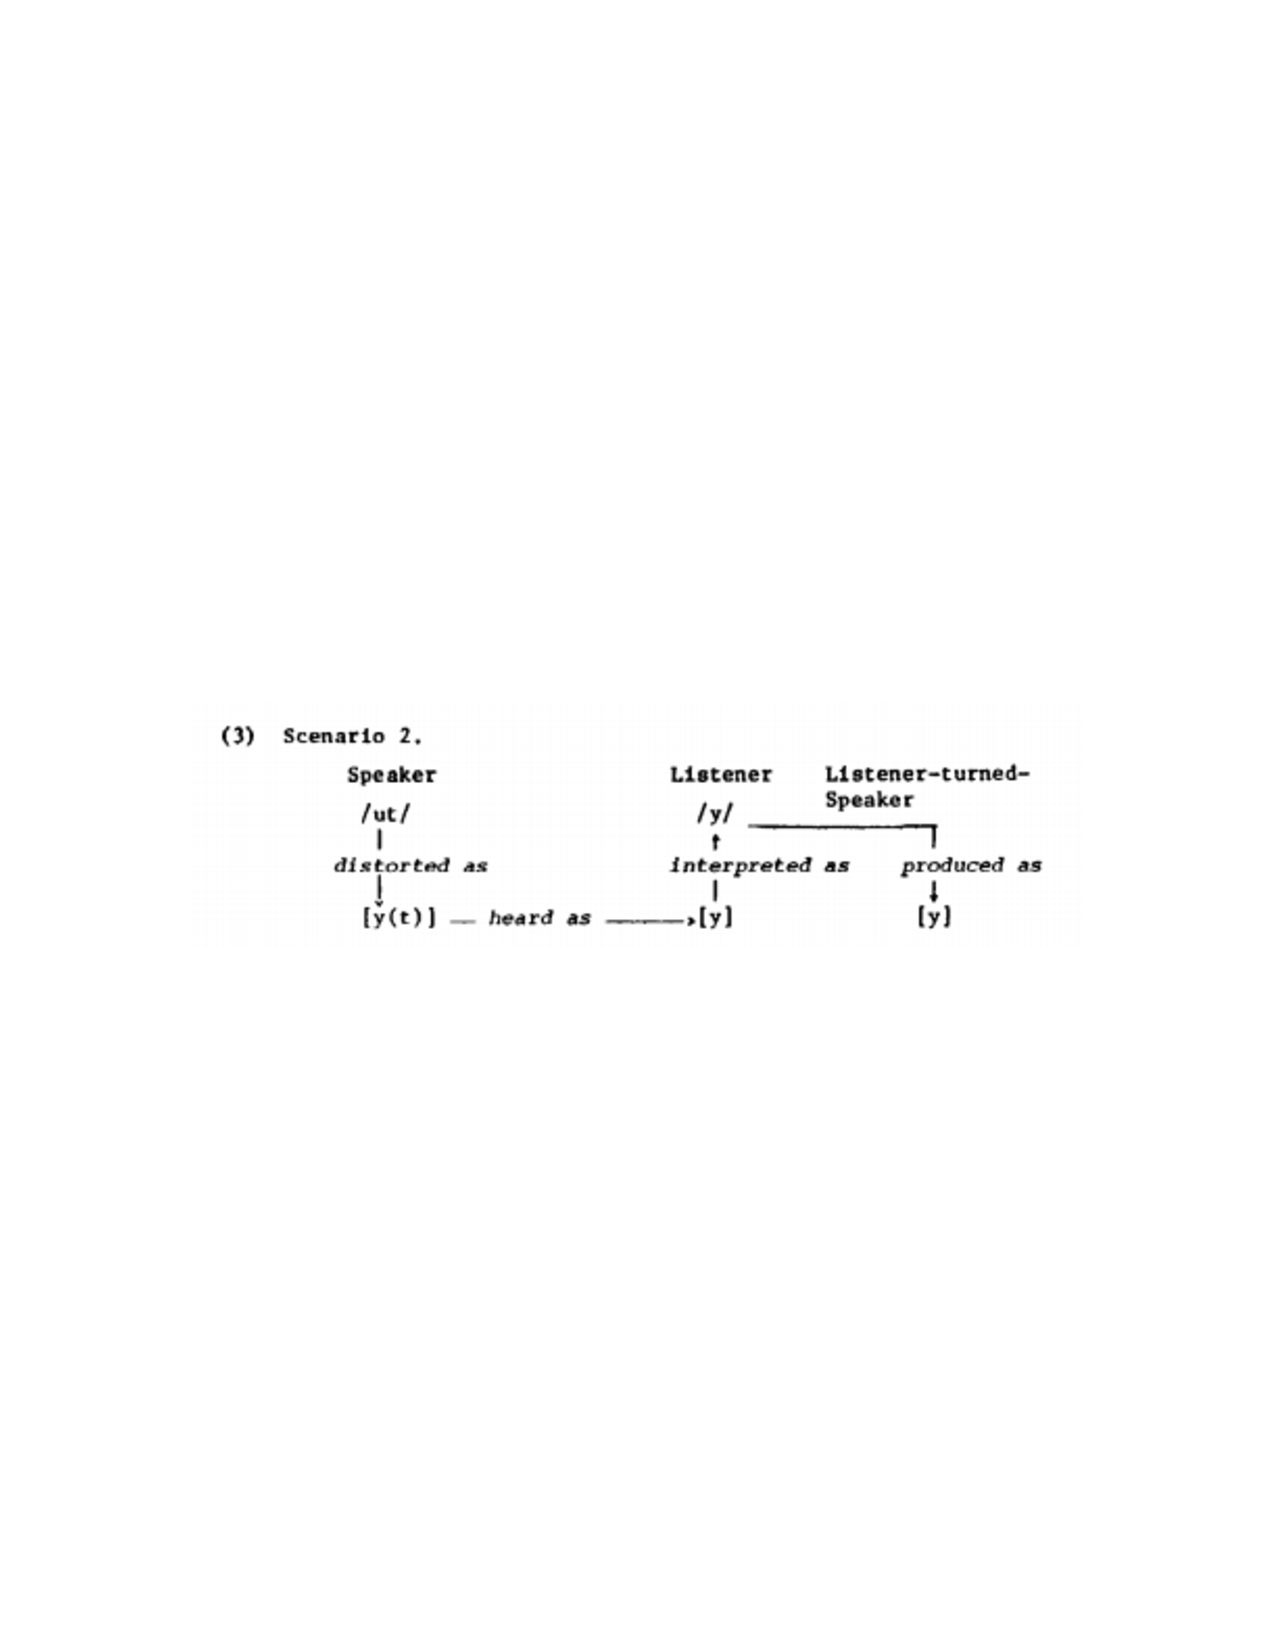
\includegraphics[trim=2cm 2cm 2cm 10cm, clip=true, width=1\textwidth]{Ohala81.pdf}
%\end{textblock*}

\end{center}
\end{frame}

%\begin{frame}{Mechanical Means}
%Traditionally assumed scenario \citep{Ohala1981} \\
%\begin{center}
%IcePaHC \small{(Wallenberg, AK Ingason, EF Sigurðsson, \& E Rögnvaldsson 2011)}
% \begin{textblock*}{125mm}(0mm,14mm)
%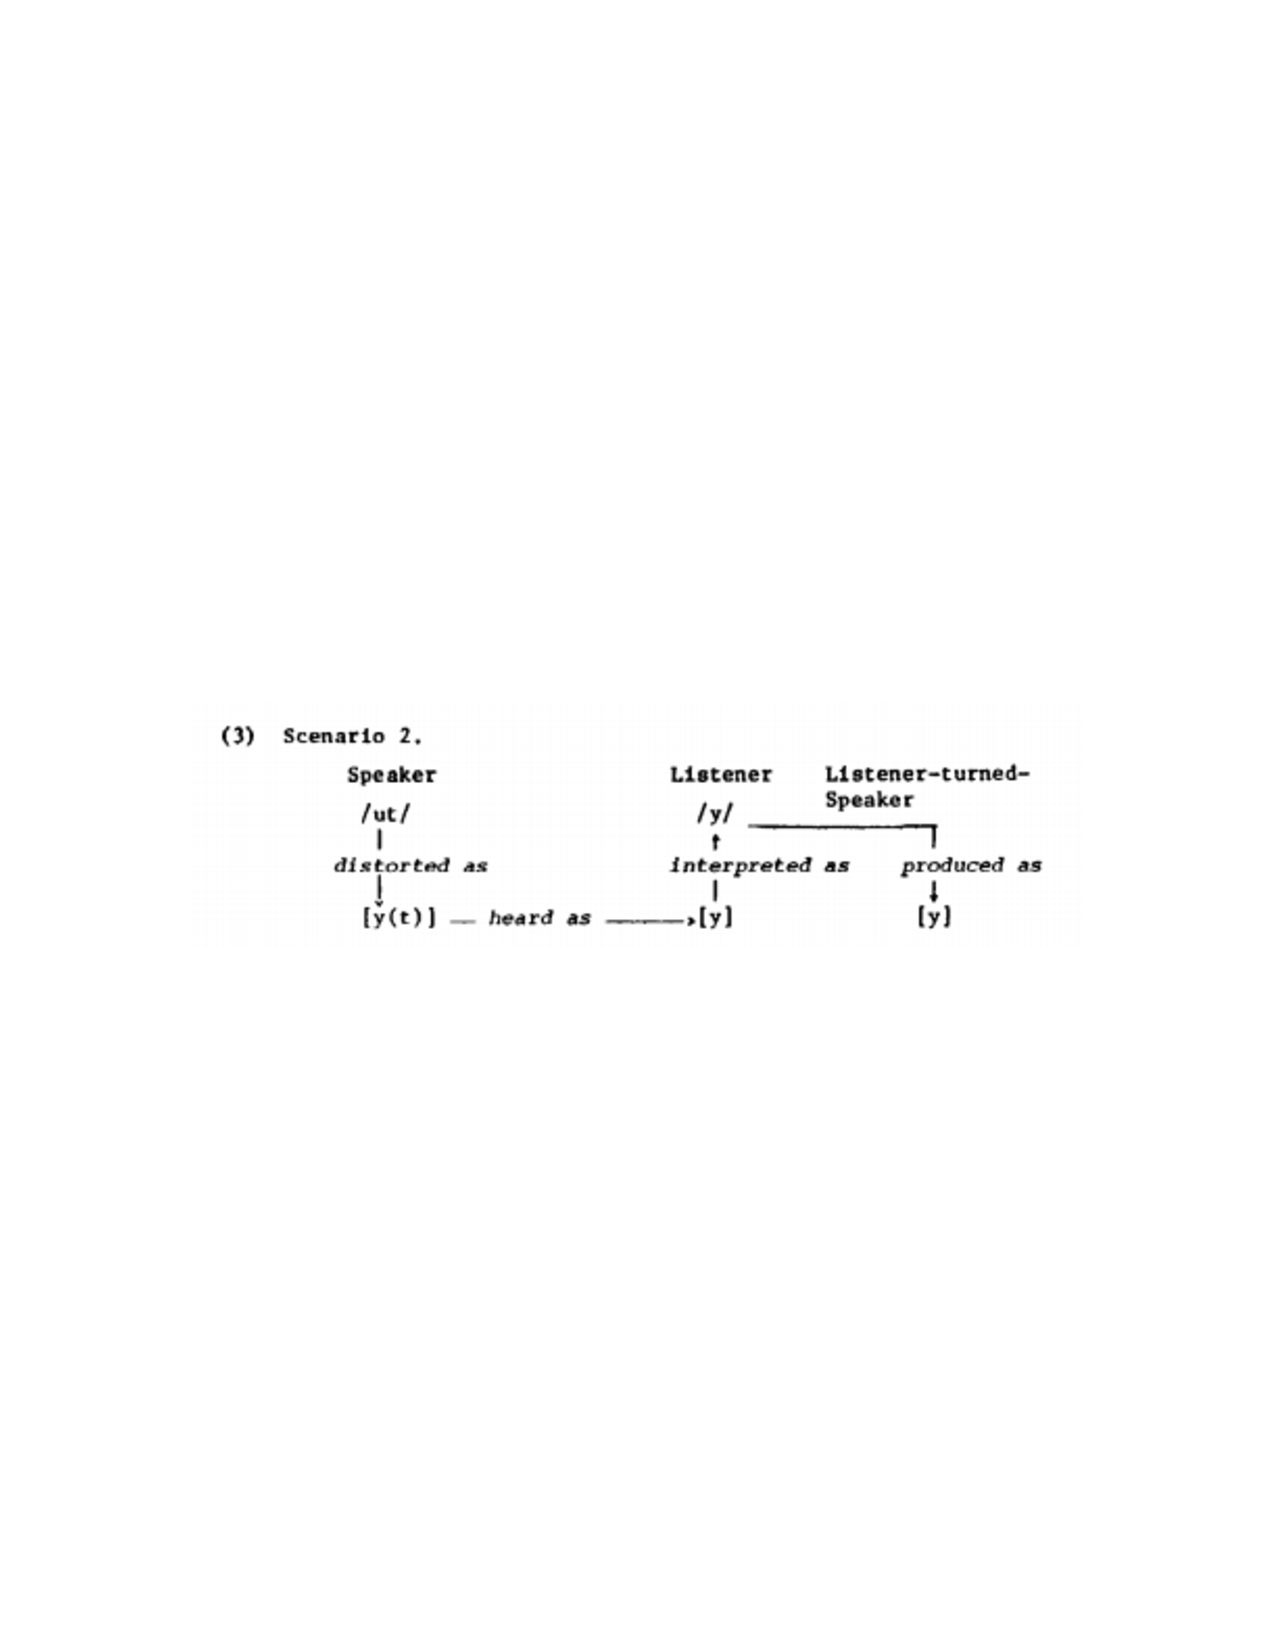
\includegraphics[trim=2cm 2cm 2cm 10cm, clip=true, width=1\textwidth]{Ohala81.pdf}
%\end{textblock*}

%\end{center}
%\end{frame}

%\begin{frame}{Clip image}
%\centering
%\includegraphics[trim=2cm 2cm 2cm 2cm,clip=true,width=5cm]{figure1}
%\end{frame}
%\begin{frame}{Mechanical Means}
	%Traditionally assumed scenario \citep{Ohala1981} 	
%	\begin{center}
%	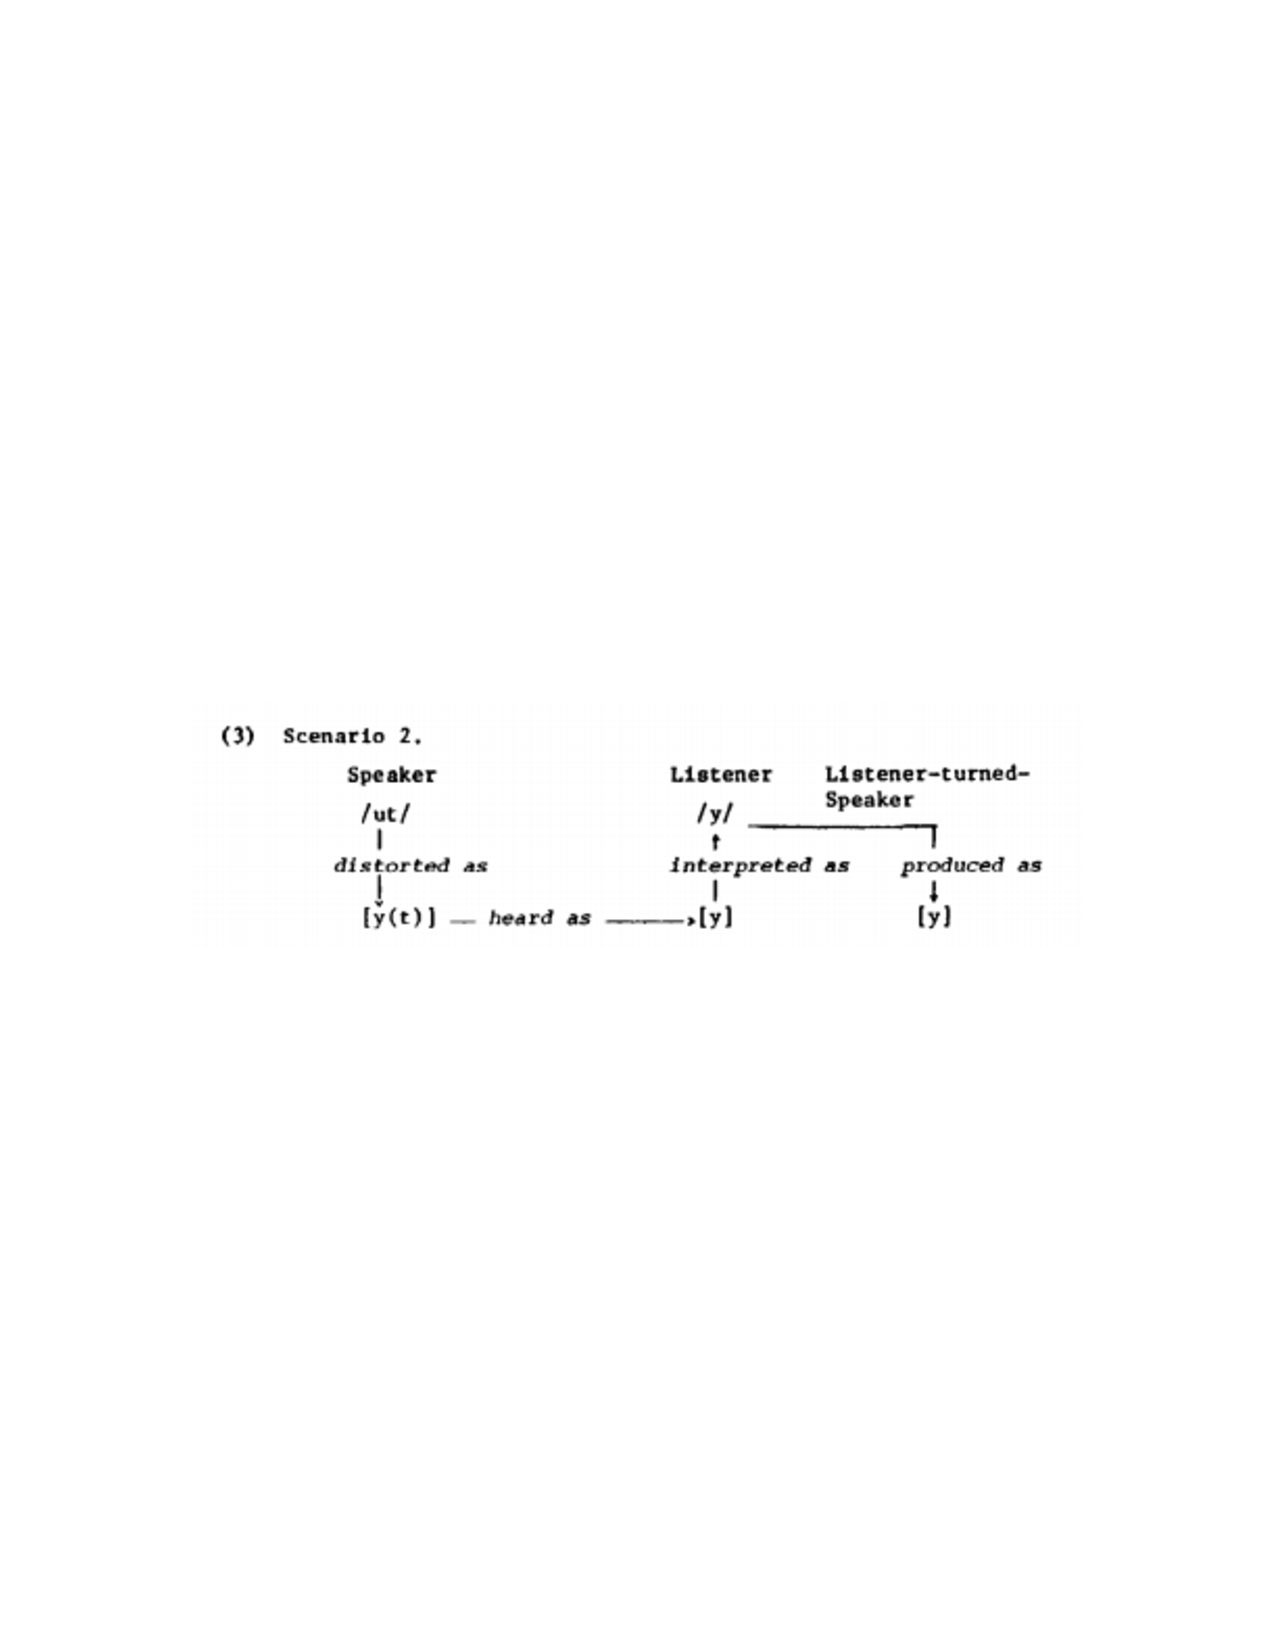
\includegraphics[width=.9\textwidth]{Ohala81.pdf}
%	\end{center}
%\end{frame}

%\subsubsection{Example: preaspiration in NW England English}}
\begin{frame}{Mechanical Means}
\begin{center}
\small{Preaspiration in Aberystwyth English \citep{Hejna2014}}

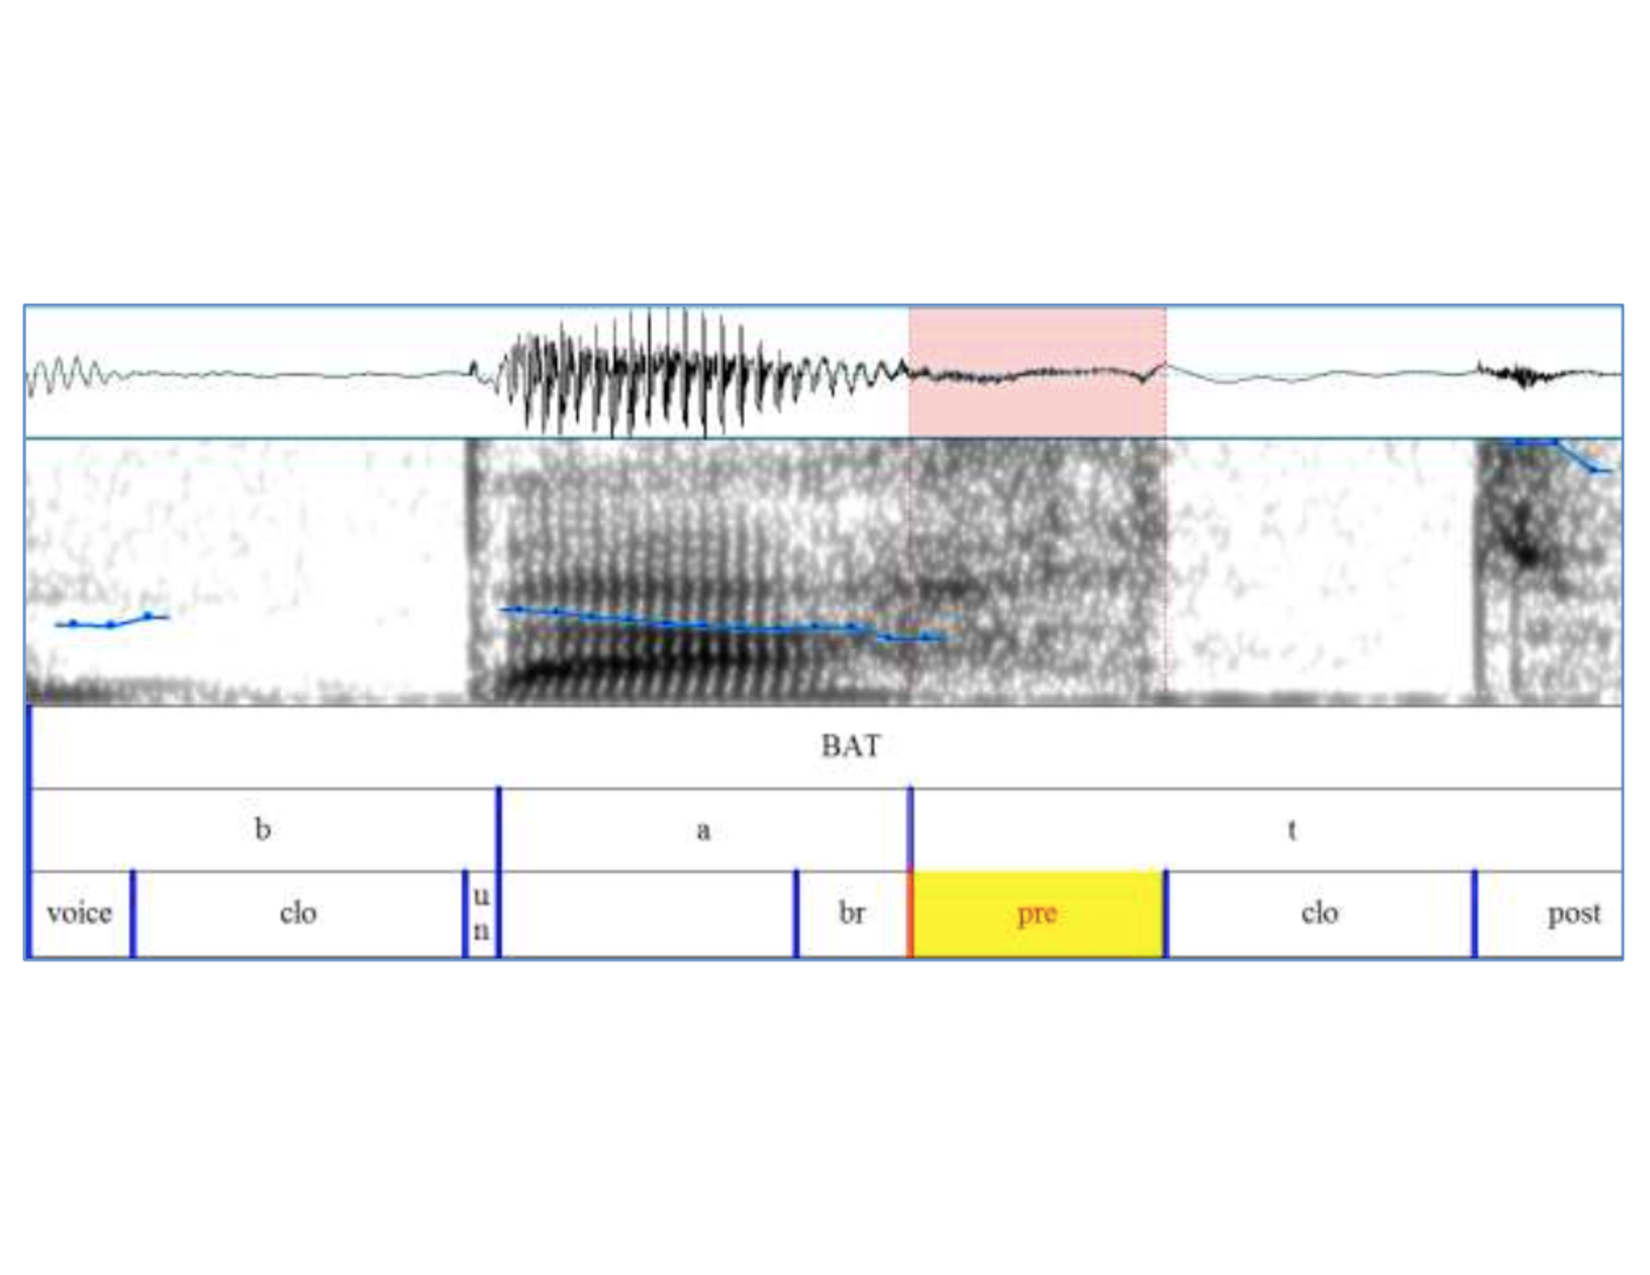
\includegraphics[trim=2cm 2cm 2cm 5cm, clip=true, width=.7\textwidth]{PreaspEx.pdf}
\end{center}
\end{frame}

\begin{frame}{Mechanical Means:  \small{Preaspiration in Aberystwyth English \citep{Hejna2014}}}
%NoteJCW: we'll need to say why we think this was phonetic and how we know it's now phonological
\begin{center}
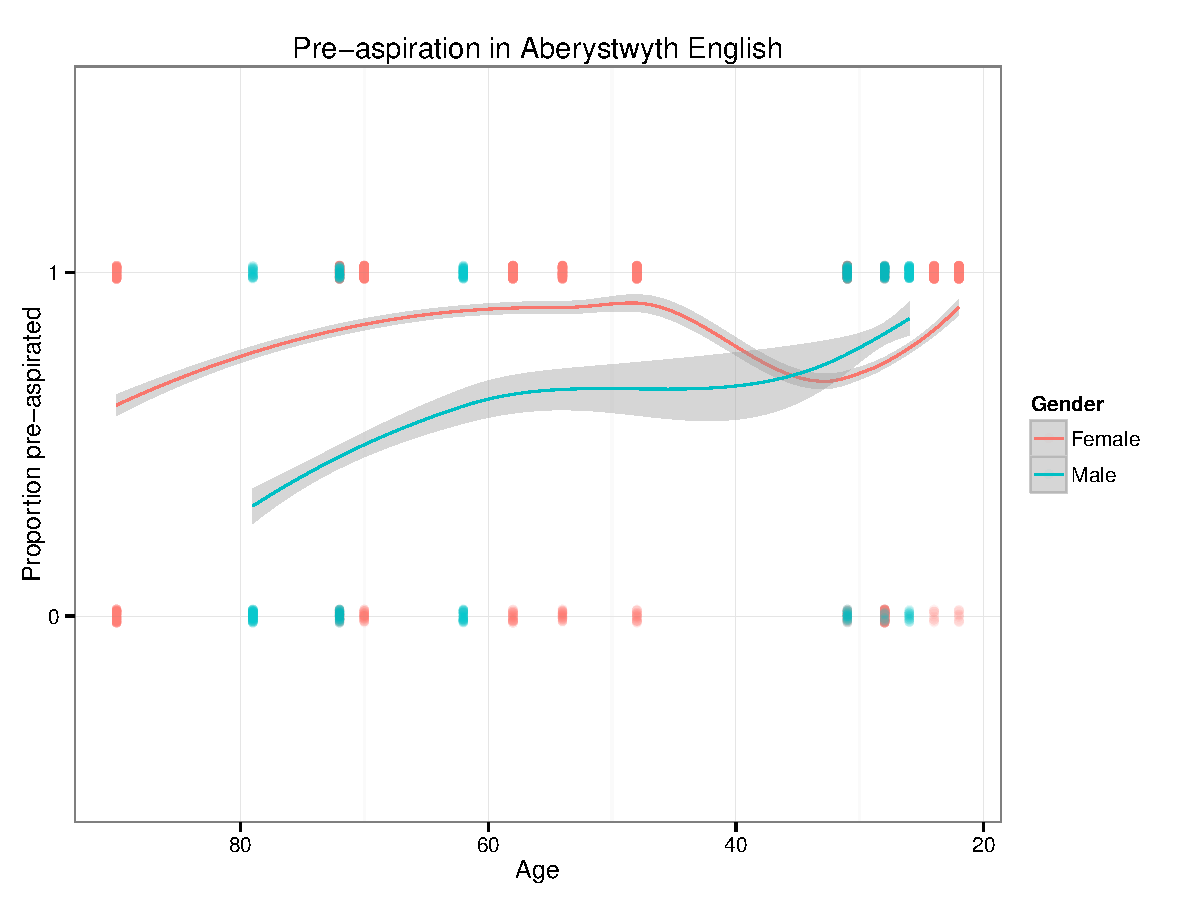
\includegraphics[trim=2cm 2cm 2cm 2cm, clip=false, width=.6\textwidth]{misaplot.pdf}
\end{center}
\end{frame}

\subsection{Spontaneous Phonologization}

\begin{frame}{Spontaneous Phonologization}
	Scenario proposed by \citet{JandaJoseph2003, fruehwald2013} 
	
	\begin{itemize}
		\item Speakers \textbf{spontaneously} create an allophone without any phonetic motivation.  \\
		\begin{itemize}
			\item Allophonic categories emerge in individual speakers' grammars before any phonetic motivation
		\end{itemize}
	\end{itemize}
\end{frame}

%\subsubsection{Example: PRICE-raising in Philadelphia English}
\begin{frame}{Spontaneous Phonologization: \\ \small{PRICE-raising in Philadelphia English (Fruehwald 2013)}}

	
\begin{center}
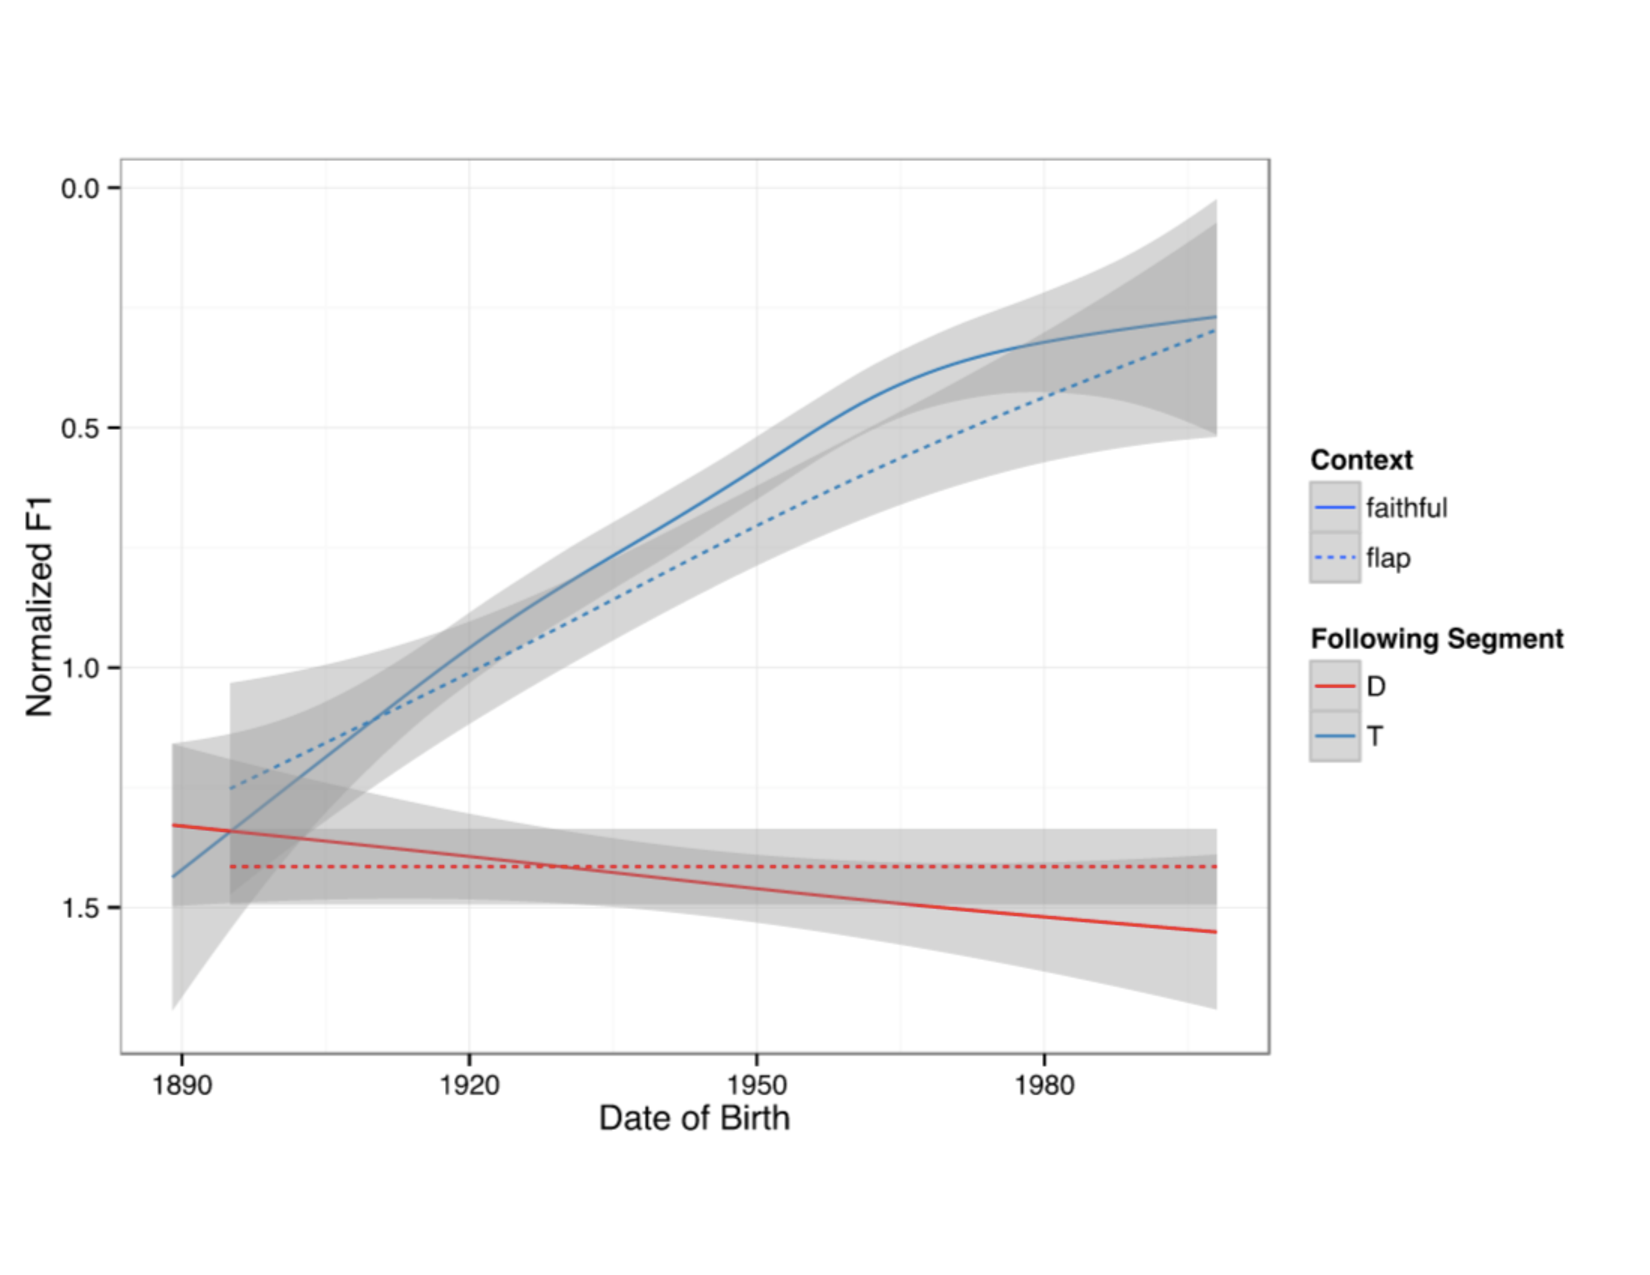
\includegraphics[trim=2cm 2cm 2cm 2cm, clip=false, width=.8\textwidth]{ayraisingphila.pdf}
\end{center}

\end{frame}

\subsection{Phonological Specialization}

\begin{frame}{Phonological Specialization}

	Proposed by us \pause
	\begin{itemize}
		\item A phonetic change begins, creating variation in phonetic space \pause
		\item This variation is reanalyzed as an allophonic distinction for a generation of speakers \pause
		\begin{itemize}
				\item Different from \citet{Ohala1981} because the phonologization is not the result of compounded perception or production errors \pause
				\item Different from \citet{fruehwald2013, JandaJoseph2003} because phonetics still play a role 
		\end{itemize}
	\end{itemize}

\end{frame}

%\subsubsection{Example: GOOSE-fronting in New Zealand English}
\begin{frame}{Phonological Specialization: \\ \small{GOOSE-NEW split in New Zealand English (Seyfarth and Sneller 2014)}}

\begin{center}
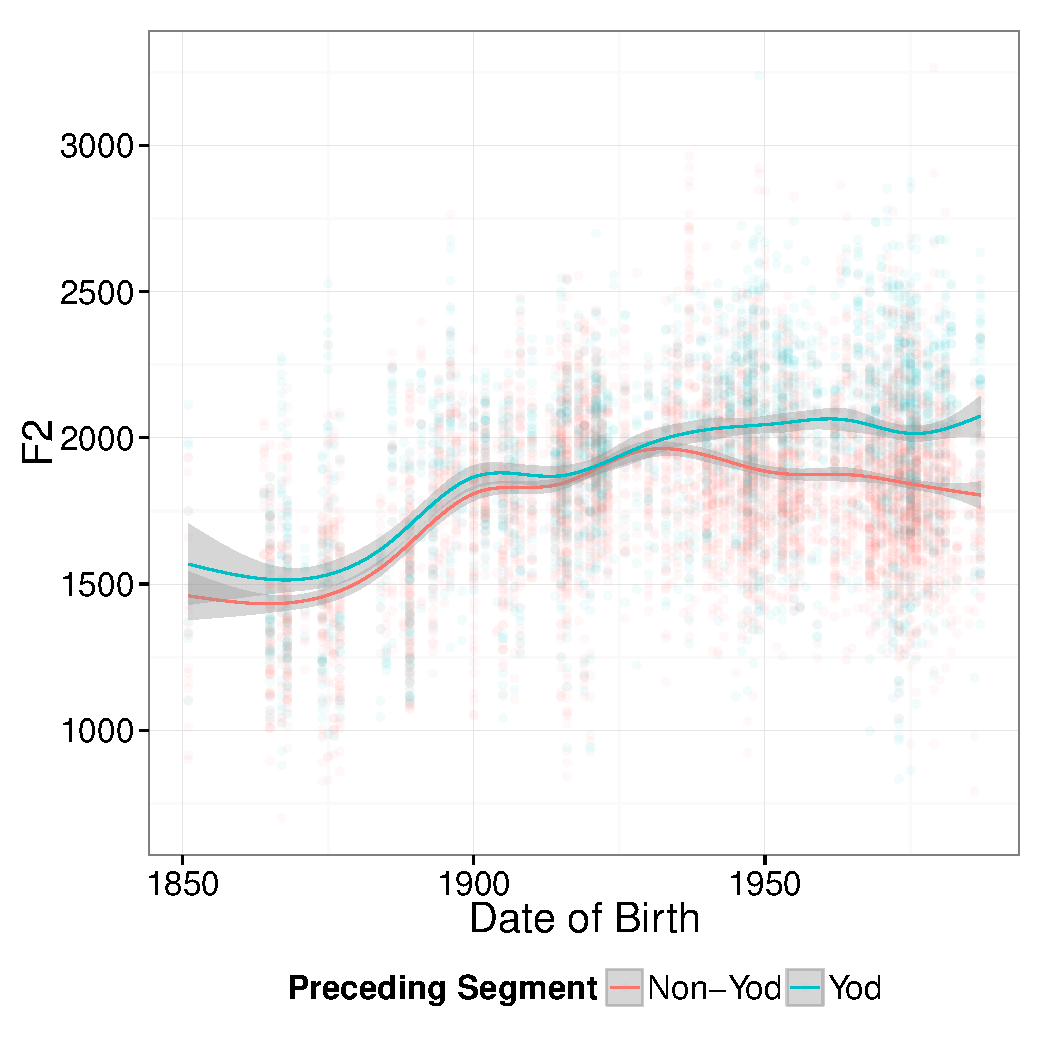
\includegraphics[width=.8\textwidth,height=.7\textheight]{ByTokenOldPreceding.pdf}
\end{center}
\end{frame}
%Note:JCW about here we should have a slide explaining the reanalysis of the community variance as two allophones' variance, and maybe compare this to categorical variation, invoking the Principle of Contrast and citing me and Joe
\section{Testing for the types}

\subsection{Effect of duration}
\begin{frame}{Effect of duration: \\ coarticulation vs. allophony}
	\begin{itemize} 
		\item If a difference in acoustic output is caused by coarticulation rather than allophony, then the difference will be bigger for shorter tokens
		\item If the difference is caused by allophony, then long and short tokens will all show a difference
	\end{itemize}
	\begin{center}

	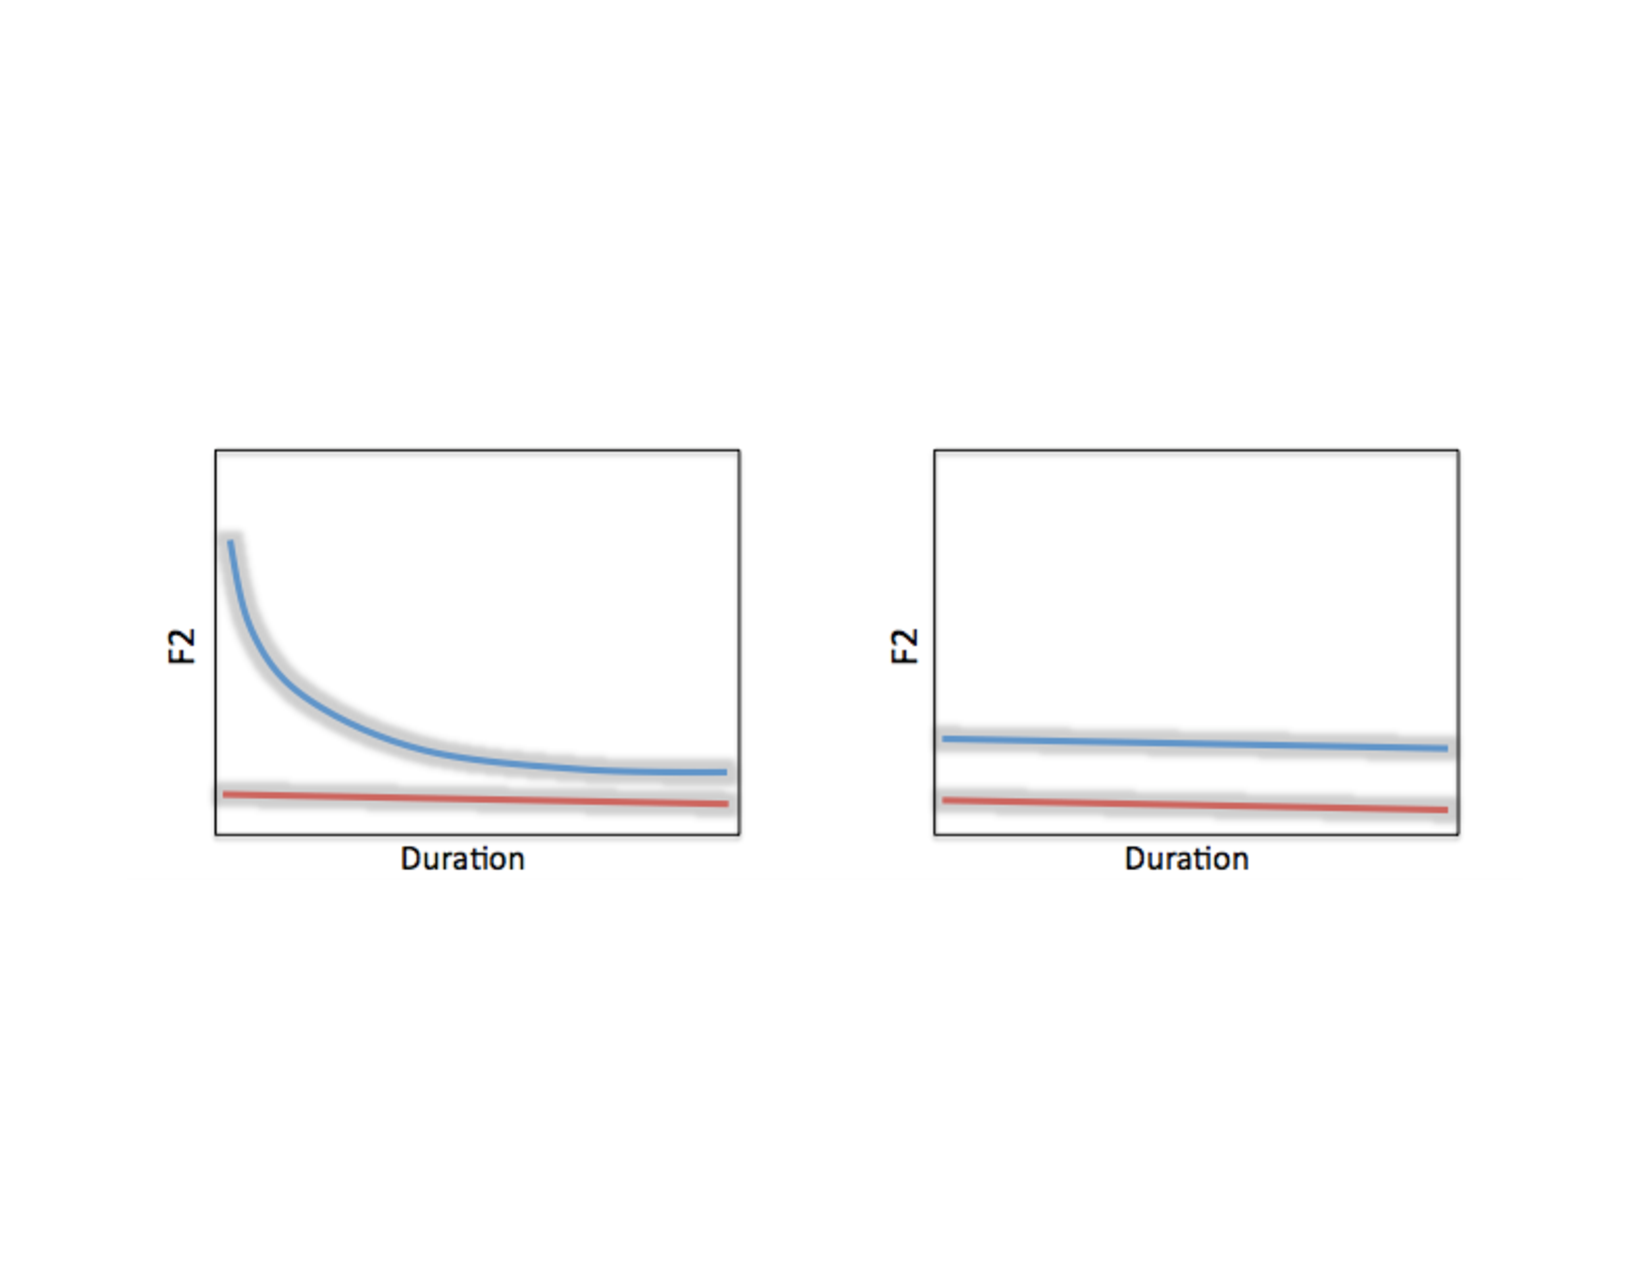
\includegraphics[trim=2cm 2cm 2cm 6cm, clip=true, width=1\textwidth]{DurationEx.pdf}

\end{center}\end{frame}

\begin{frame}{Effect of duration: Mechanical means}
%NoteJCW: I added another point below
	\begin{block}{Mechanical means}
		\begin{itemize}
			\item Because the allophonic split is the result of accruing phonetic effects, we should see an effect of duration for most speakers, until a reanalysis has been made.
			\item After the reanalysis, as the new allophone spreads, the earlier effect of duration should decrease over time.
		\end{itemize}
	\end{block}	
\end{frame} 

\begin{frame}{Effect of duration: Mechanical means}
	\begin{block}{Mechanical means}
		\begin{center}
		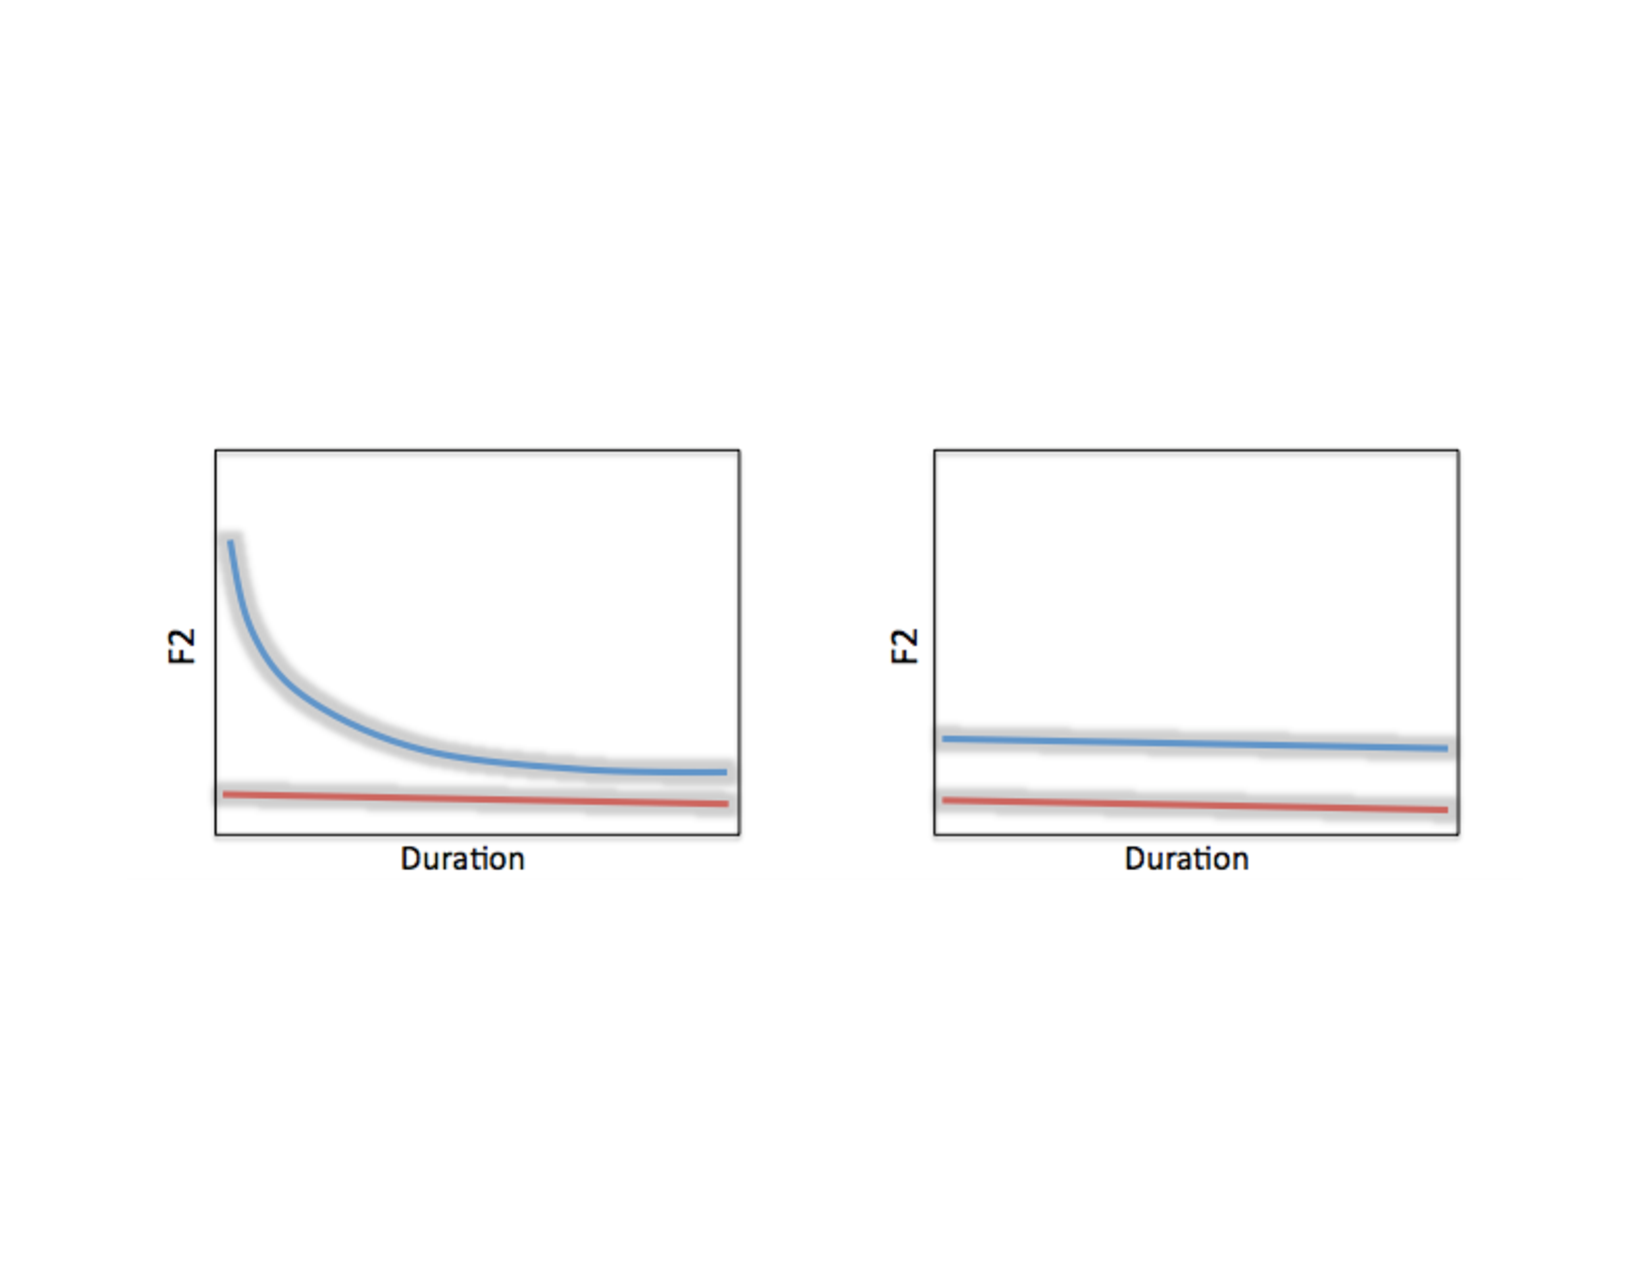
\includegraphics[trim=2cm 2cm 2cm 2cm, clip=false, width=.7\textwidth]{DurationEx.pdf}
		\end{center}
	\end{block}	
\end{frame}

\begin{frame}{Effect of duration: Spontaneous phonologization}
	\begin{block}{Spontaneous phonologization}
		\begin{itemize}
			\item Because there is no phonetic effect that precedes the phonological effect, we should see no effect of duration at any time \pause
			\begin{xlist}
				\ex Speakers with one category show no coarticulation (no difference to be found) \pause
				\ex Speakers with two categories show two phonological categories (no effect of duration) 
			\end{xlist}
		\end{itemize}
	\end{block}	
\end{frame}

\begin{frame}{Effect of duration: Spontaneous phonologization}
	\begin{block}{Spontaneous phonologization}
	\begin{center}
	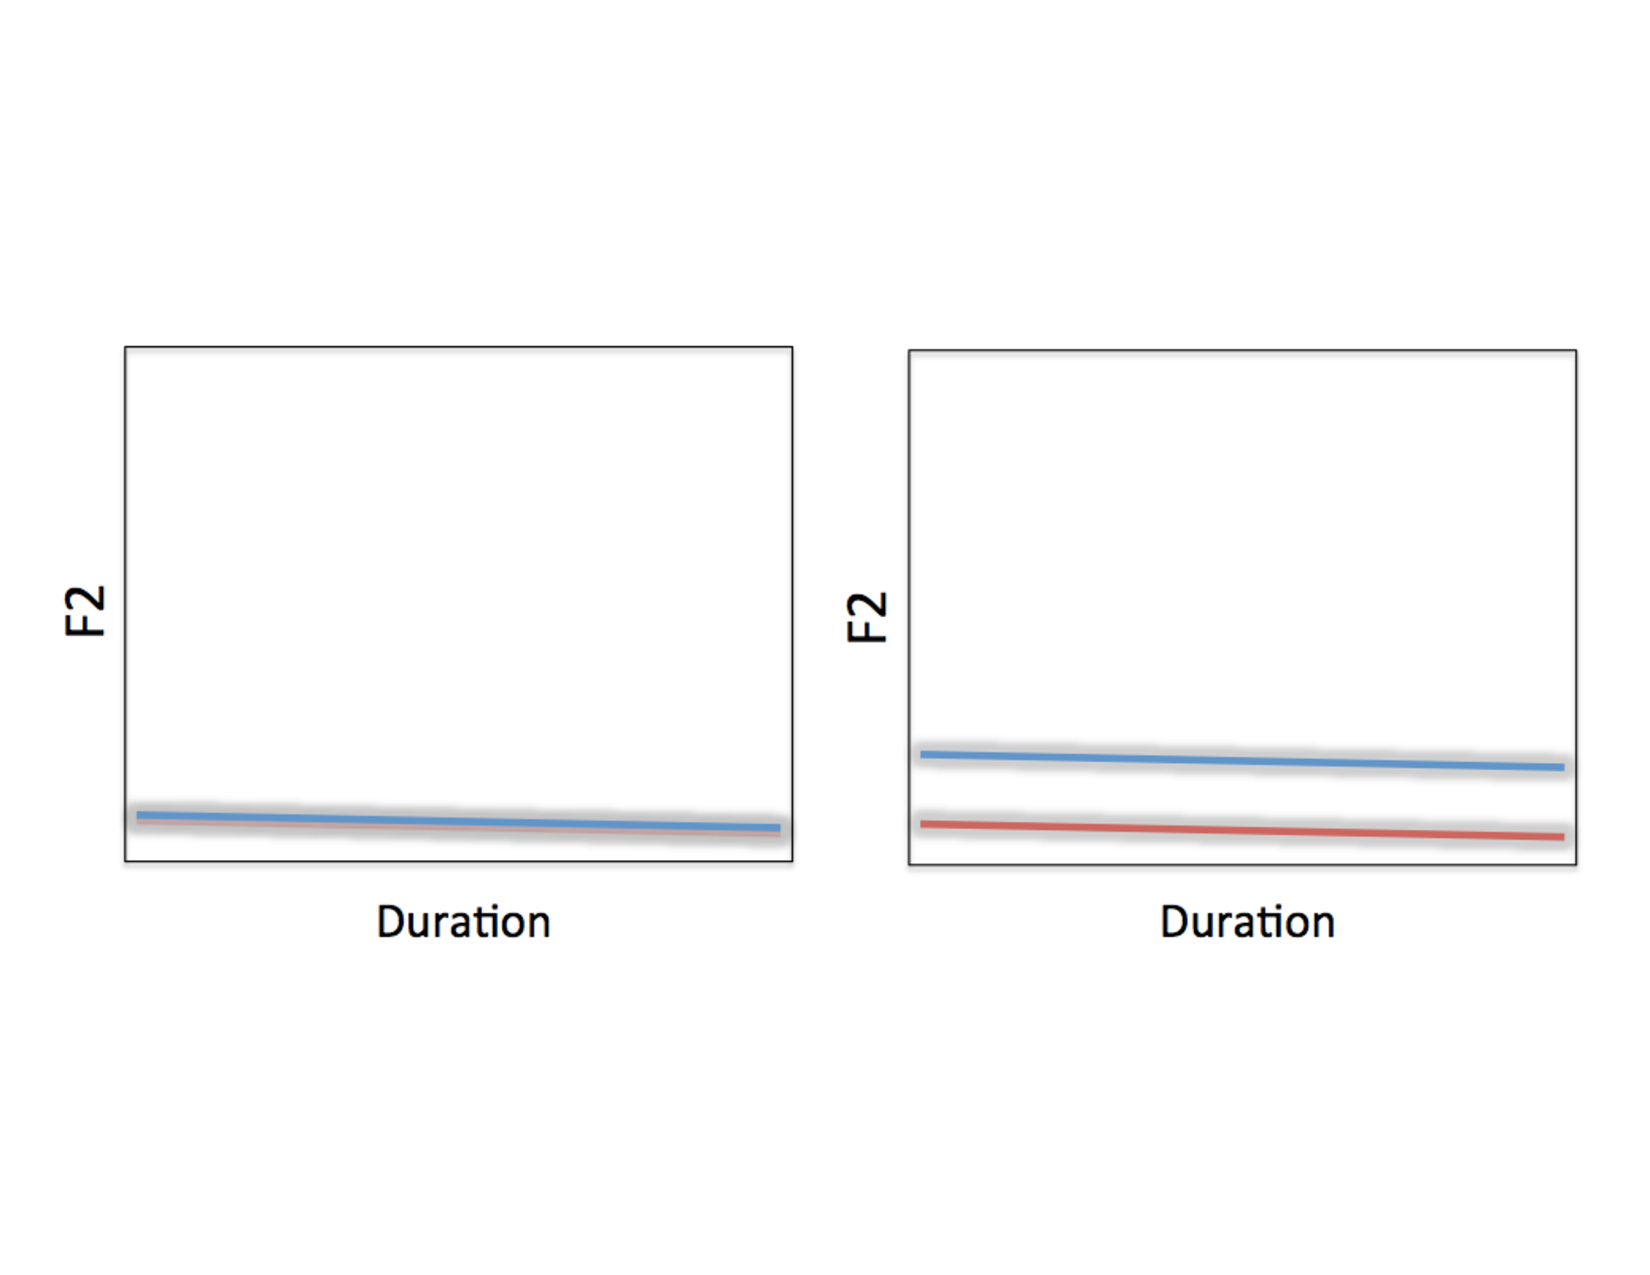
\includegraphics[trim=2cm 2cm 2cm 2cm, clip=false, width=.7\textwidth]{spontdurex.pdf}
	\end{center}
	\end{block}	
\end{frame}

\begin{frame}{Effect of duration: Phonological specialization}
	\begin{block}{Phonological specialization}
		\begin{itemize}
			\item Because the phonologization is the result of reanalyzed coarticulation, we should see older speakers showing an effect of duration (shorter tokens more distinct) \pause
			\item and younger speakers with two distinct categories for tokens of all duration
		\end{itemize}
	\end{block}	
\end{frame}

\begin{frame}{Effect of duration: Phonological specialization}
	\begin{block}{Phonological specialization}
	\begin{center}
	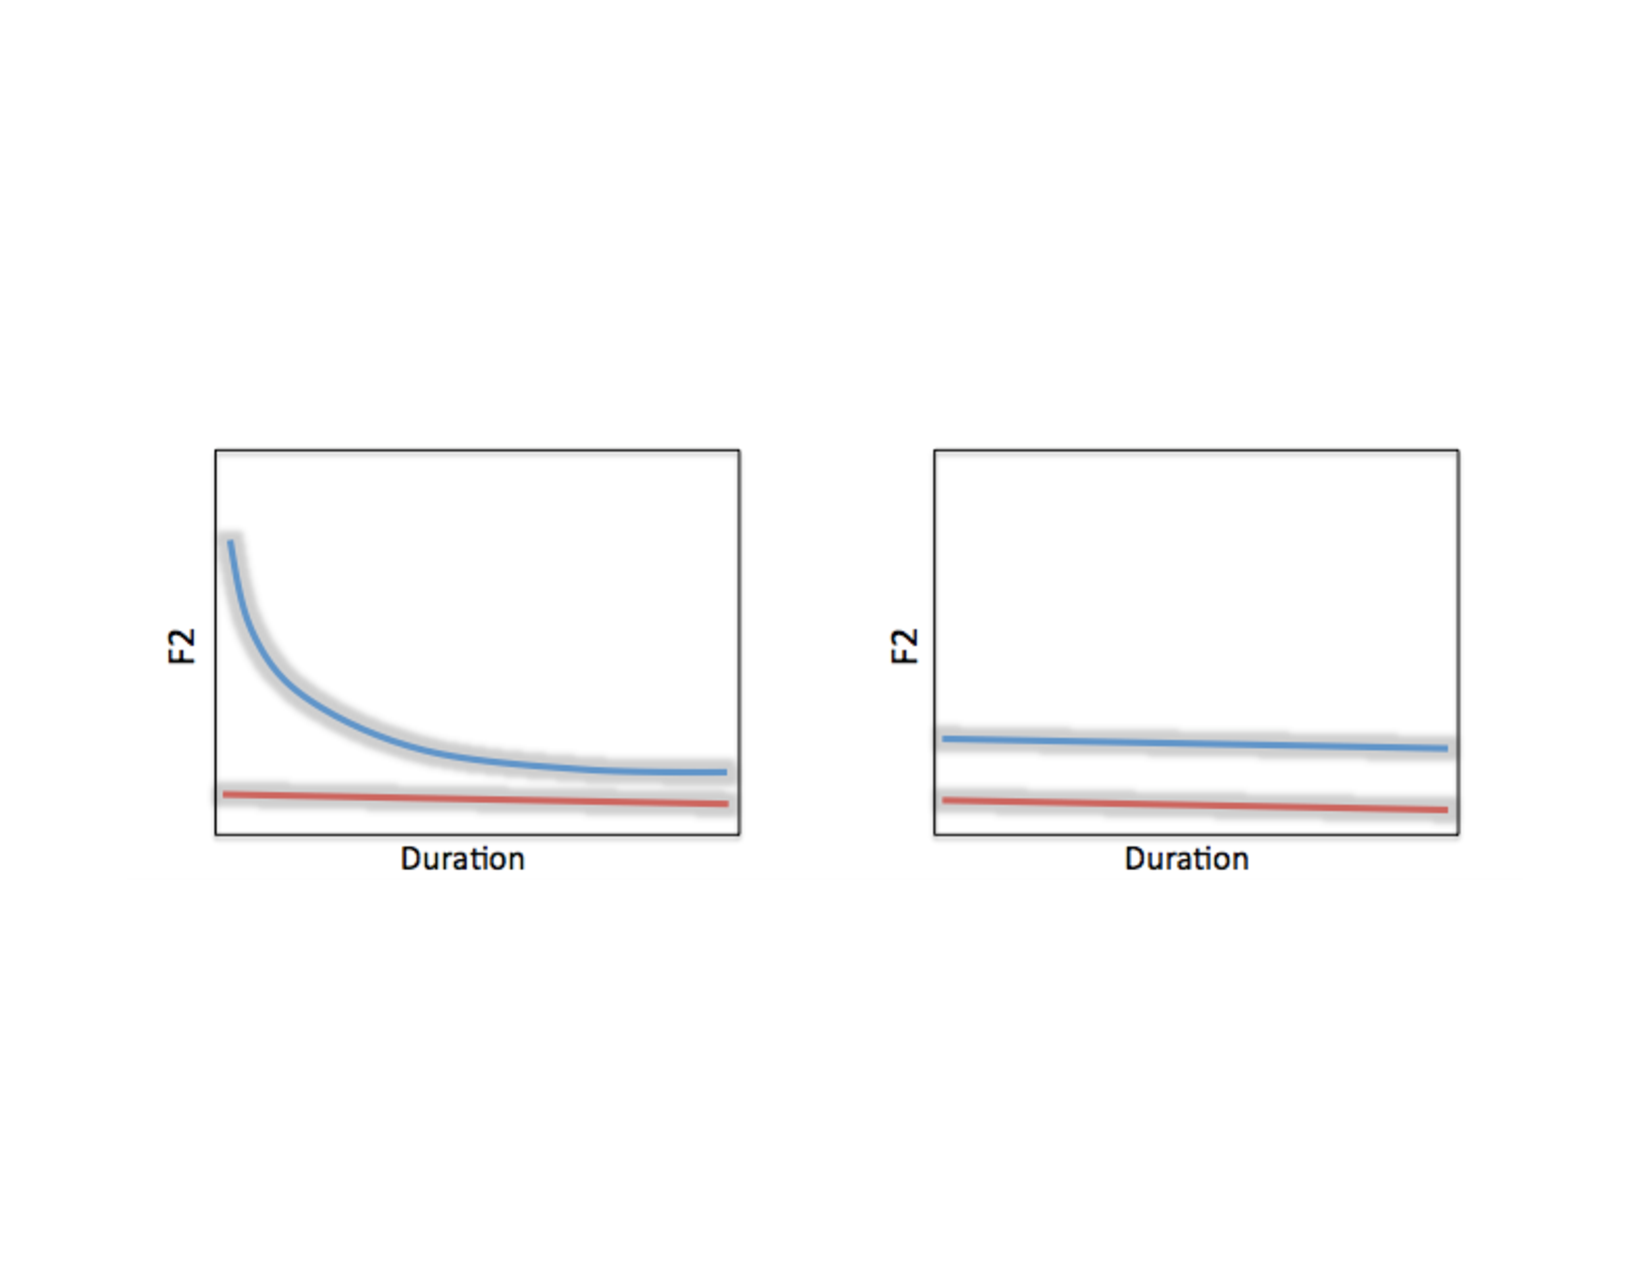
\includegraphics[trim=2cm 2cm 2cm 2cm, clip=false, width=.7\textwidth]{DurationEx.pdf}
	\end{center}
	\end{block}	
\end{frame}

\begin{frame}{Effect of duration: Phonological specialization}
	\begin{block}{Phonological specialization in New Zealand English /u/-fronting}
	\begin{columns}[c]
	\column{.5\textwidth}
	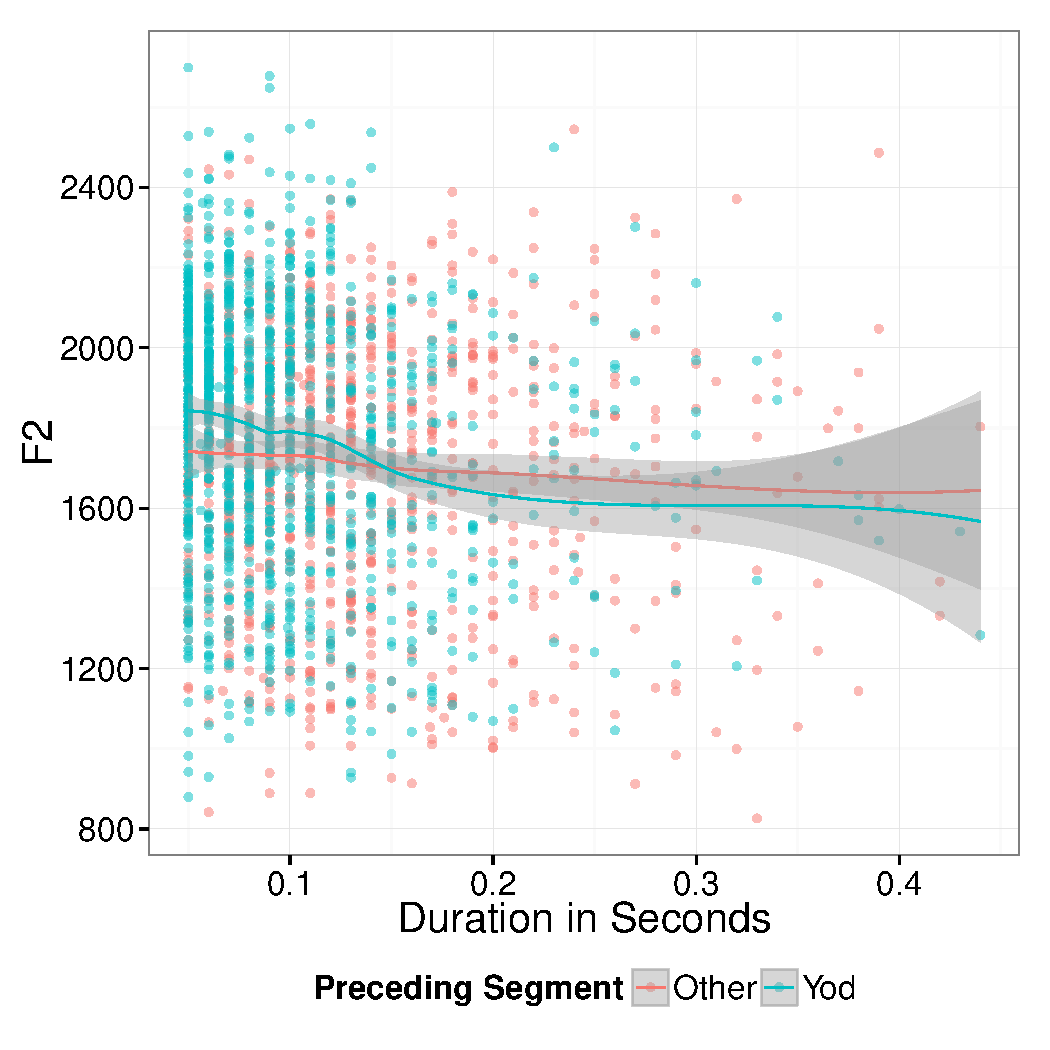
\includegraphics[trim=2cm 2cm 2cm 2cm, clip=false, width=.7\textwidth]{GooseNewOldDur.pdf}
	\column{.5\textwidth}
	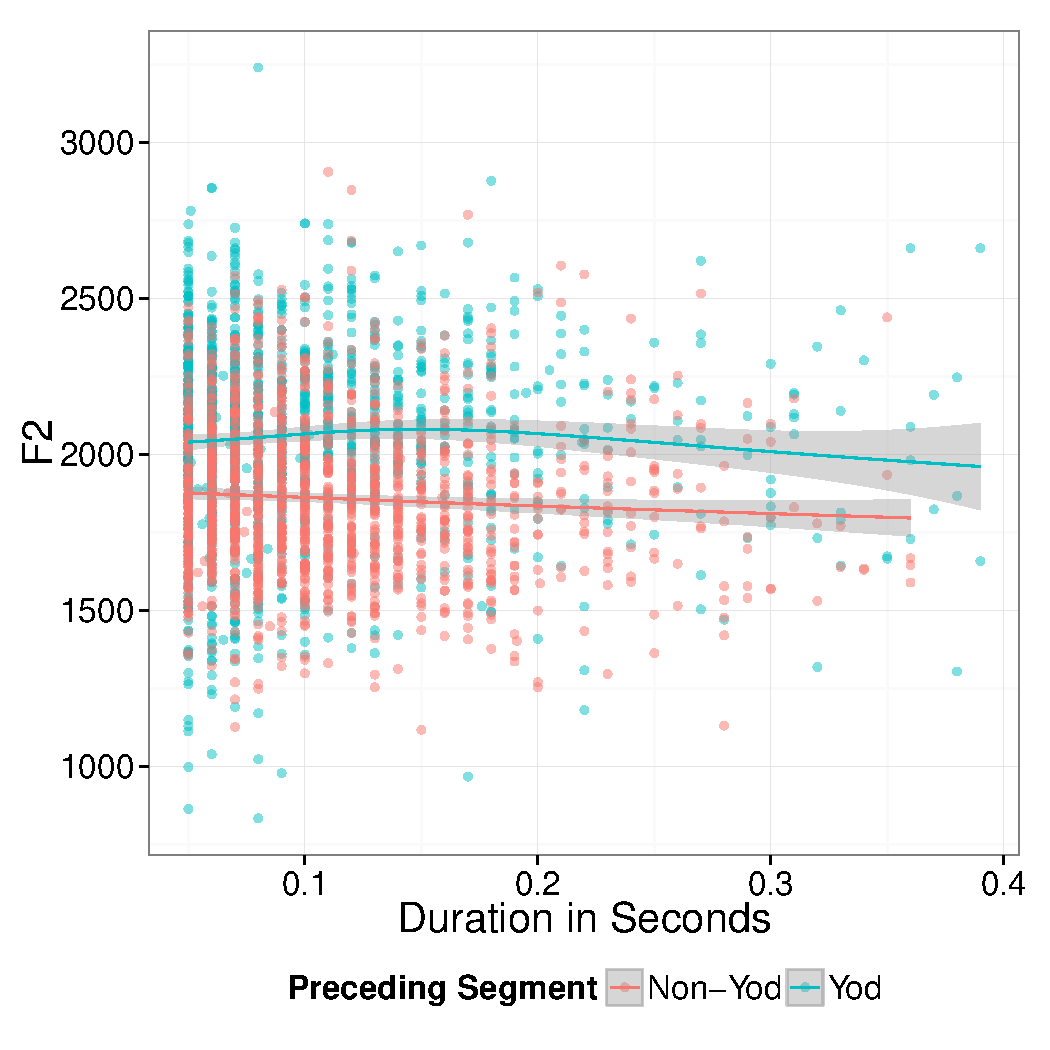
\includegraphics[trim=2cm 2cm 2cm 2cm, clip=false, width=.7\textwidth]{GooseNewYoungDur.pdf}
	\end{columns}
	\end{block}	
\end{frame}




%\begin{frame}{Conclusions}
%\begin{block}{Conclusions}
%	\begin{itemize}
%		\item Within syntax, only one formal account of optionality is available, the same one that accounts for language change: Competing Grammars.
%		\item This results in replacement, specialization, or stable variation (true optionality).
%		\item The latter is (only) the result of mapping categorical variation onto a continuous dimension of specialization.
%		\item An acquisition simulation shows how stable variation can emerge under a minimal Principle of Contrast.
%		\item It is possible and desirable to extend this formal account to other domains of variation, like morphology and phonology.
%	\end{itemize}
%\end{block}
%
%
%\end{frame}

\subsection{Rate of change}
\begin{frame}{Rate of change: coarticulation}
	\begin{itemize} 
		\item A phonological rule operates on a single phonological category \citep{fruehwald2013} \pause
		\item If two variables have different rates of change, it means there are two rules at work \pause

	\end{itemize}
	\begin{center}

	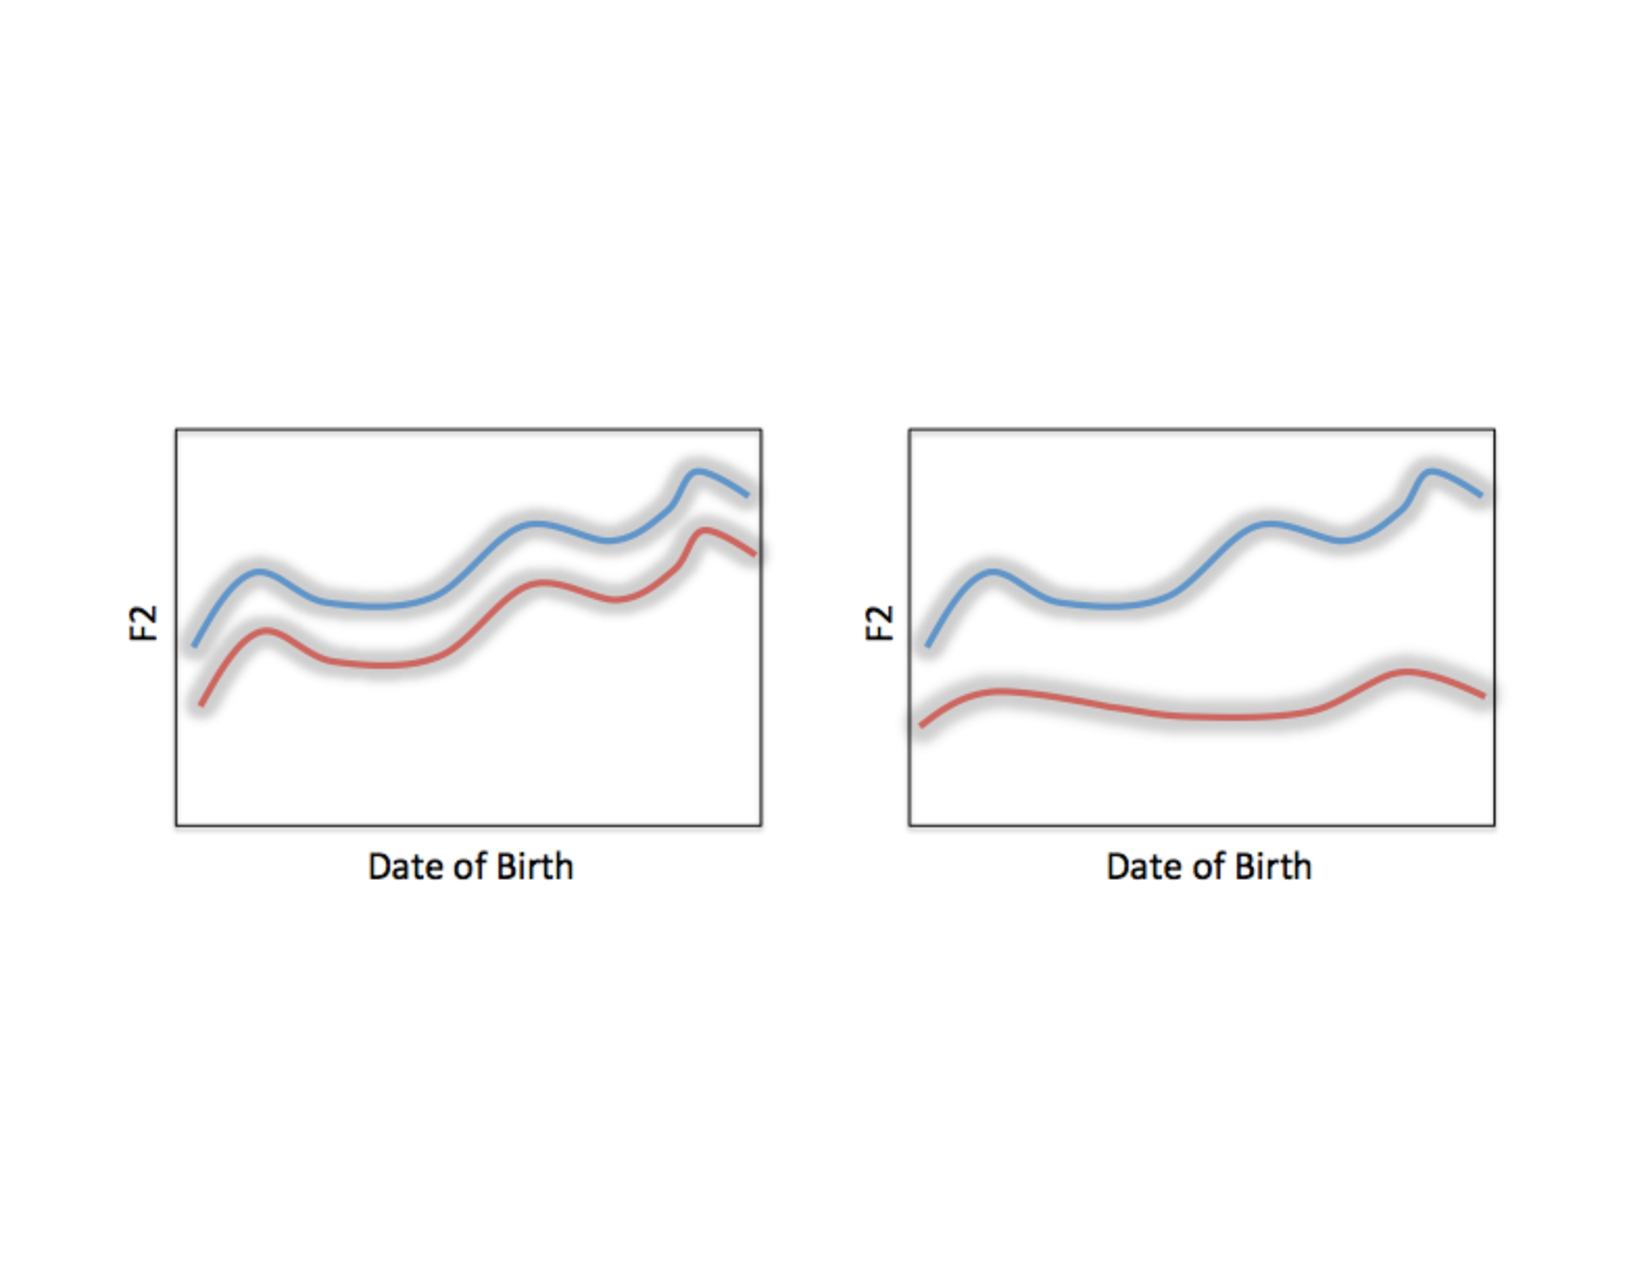
\includegraphics[trim=2cm 2cm 2cm 6cm, clip=true, width=1\textwidth]{RateofChangeEx.pdf}

\end{center}\end{frame}

\begin{frame}{Rate of change: Mechanical means}
	\begin{block}{Mechanical means}
		\begin{itemize}
			\item Because the allophonic split is the result of accruing phonetic effects, we should see a gradual drift in the two variables
		\end{itemize}
	\end{block}	
\end{frame}

\begin{frame}{Rate of change: Mechanical means}
	\begin{block}{Mechanical means}
		\begin{center}
		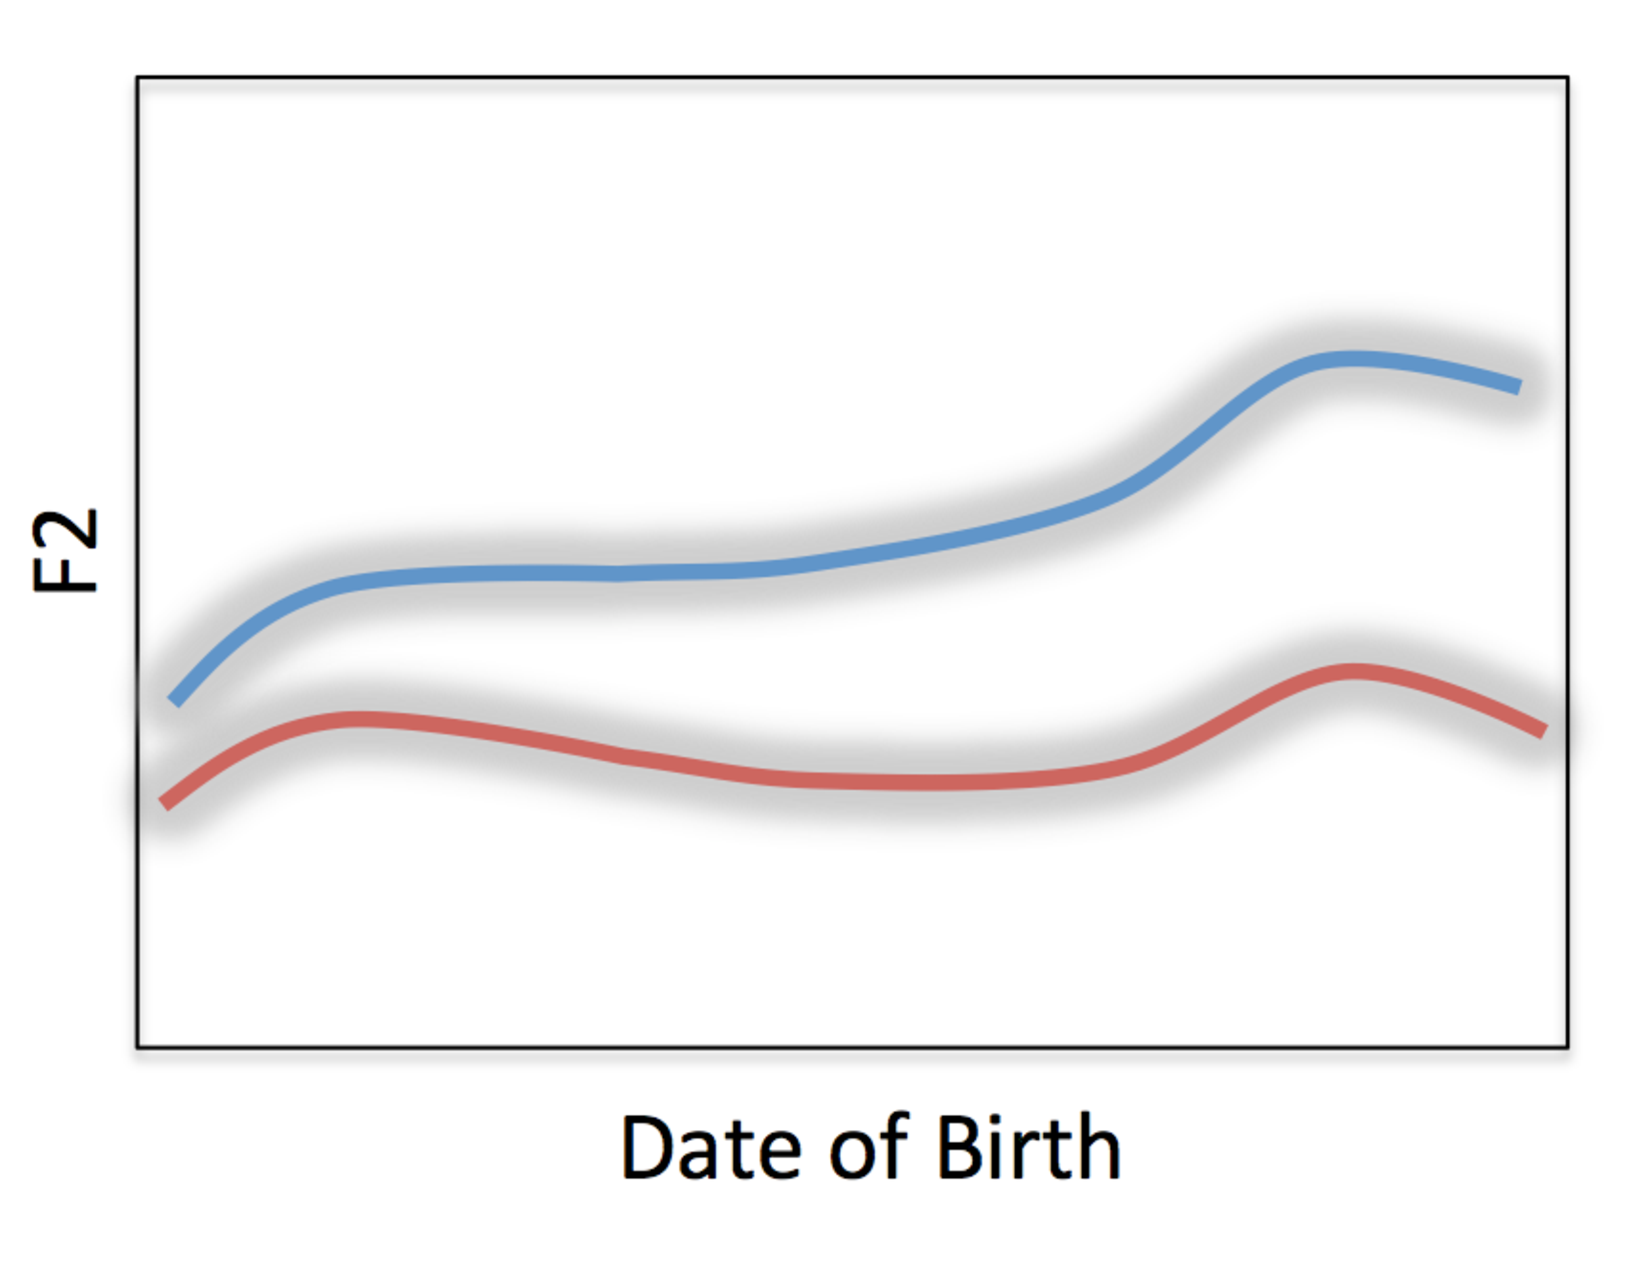
\includegraphics[trim=2cm 2cm 2cm 2cm, clip=false, width=.6\textwidth]{MechROC.pdf}
		\end{center}
	\end{block}	
\end{frame}

\begin{frame}{Rate of change: Spontaneous phonologization}
	\begin{block}{Spontaneous phonologization}
		\begin{itemize}
			\item Because the allophonic split occurs suddenly, we should see both variables in lock step until the community spontaneously creates a new category 
		\end{itemize}
	\end{block}
\end{frame}

\begin{frame}{Rate of change: Spontaneous phonologization}
	\begin{block}{Spontaneous phonologization}
		\begin{center}
		\includegraphics[trim=2cm 2cm 2cm 2cm, clip=false, width=.6\textwidth]{SpontROC.pdf}
		\end{center}
	\end{block}	
\end{frame}

\begin{frame}{Rate of change: Phonological specialization}
	\begin{block}{Phonological specialization}
		\begin{itemize}
			\item Because the allophonic split occurs suddenly, we should see both variables in lock step until the community spontaneously creates a new category \pause
			\item However, we may still see an effect of coarticulation for the early speakers
		\end{itemize}
	\end{block}
\end{frame}

\begin{frame}{Rate of change: Phonological specialization}
	\begin{block}{Phonological specialization}
		\begin{center}
		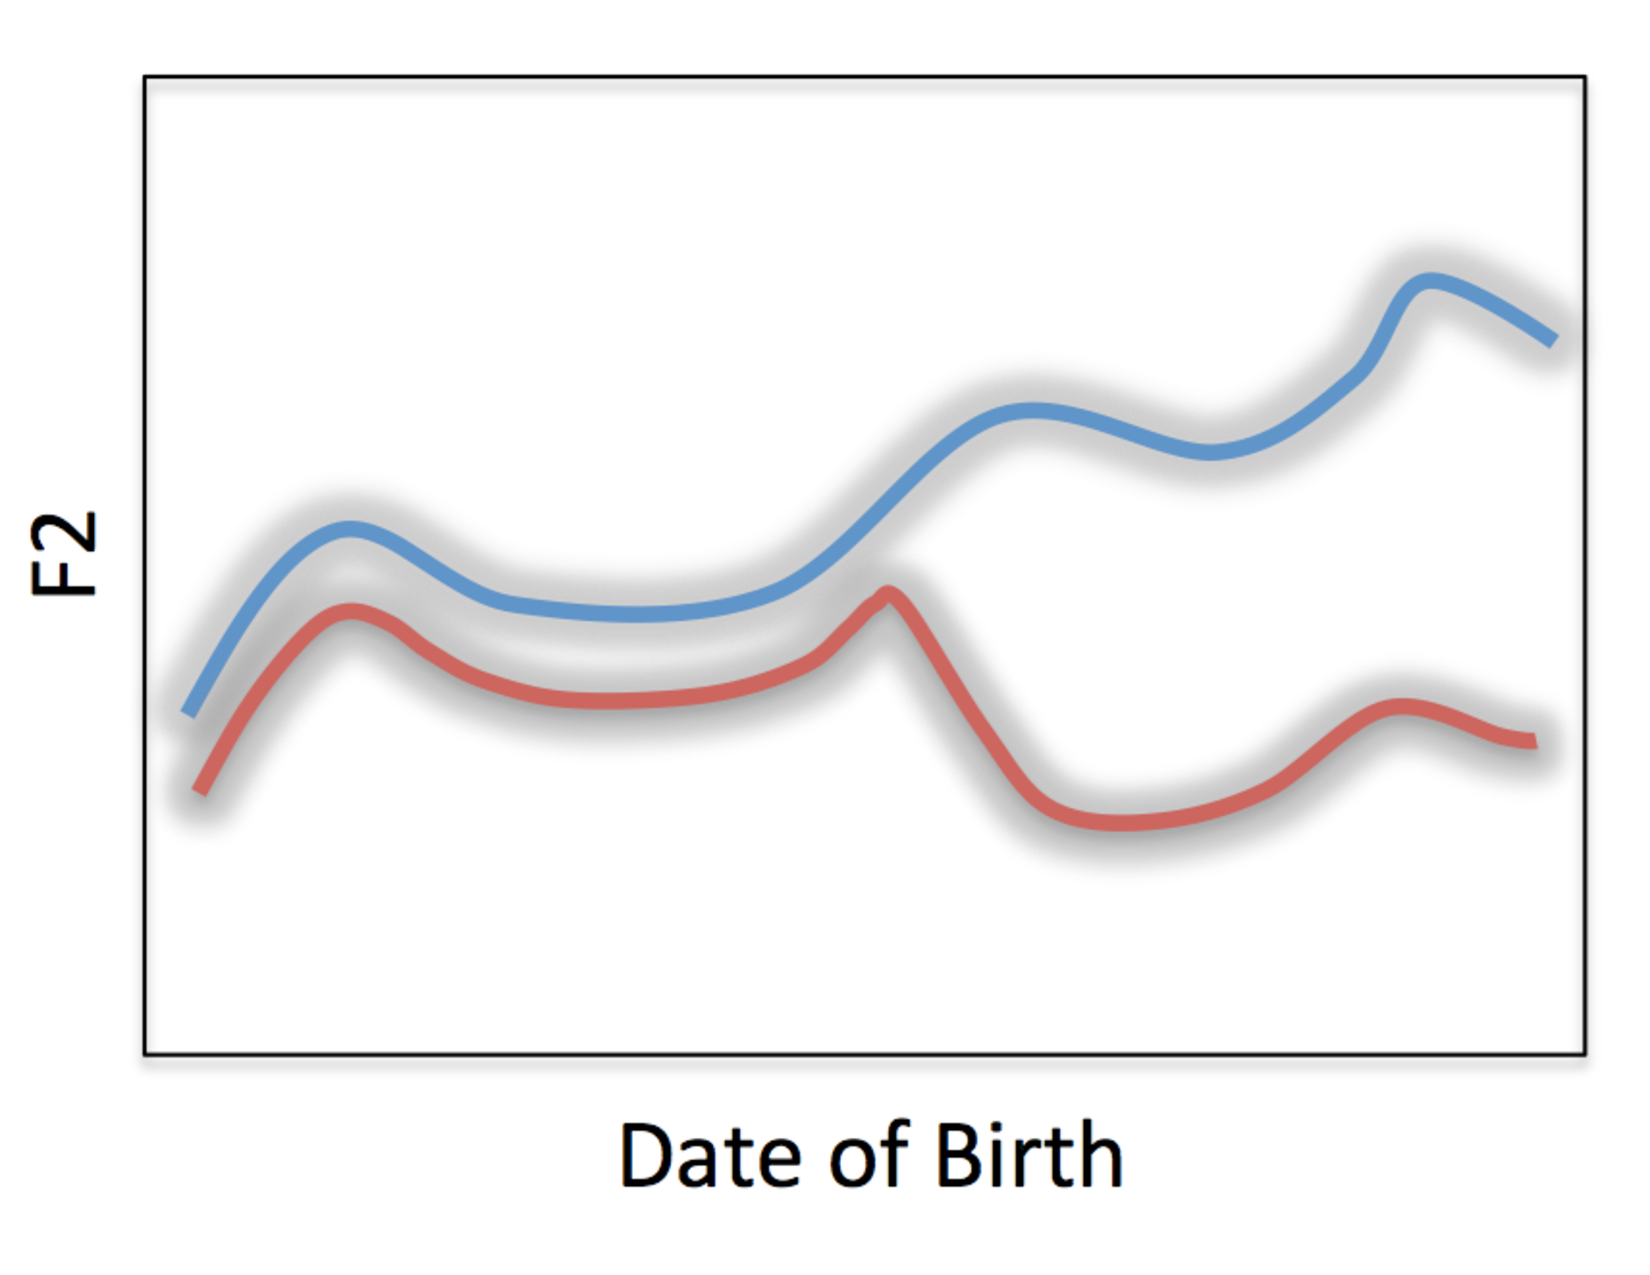
\includegraphics[trim=2cm 2cm 2cm 2cm, clip=false, width=.6\textwidth]{phonspROC.pdf}
		\end{center}
	\end{block}	
\end{frame}

\begin{frame}{Rate of change: Phonological specialization}
	\begin{block}{\small{Phonological specialization in New Zealand English /u/-fronting}}
	\begin{center}
	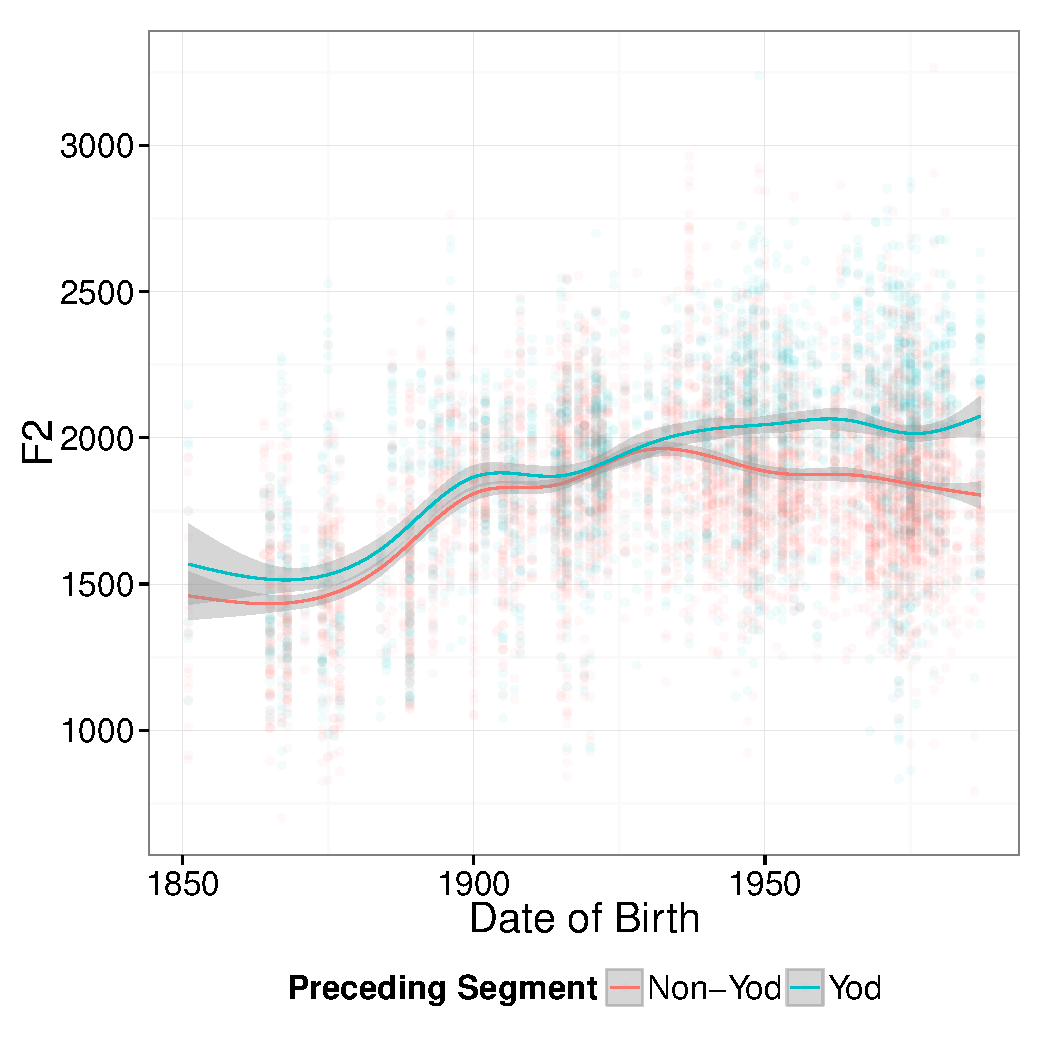
\includegraphics[width=.8\textwidth,height=.7\textheight]{ByTokenOldPreceding.pdf}
	\end{center}
	\end{block}	
\end{frame}

\begin{frame}{Rate of change: Phonological specialization}
	\begin{block}{\small{Phonological specialization in New Zealand English /u/-fronting}}
	\begin{center}
	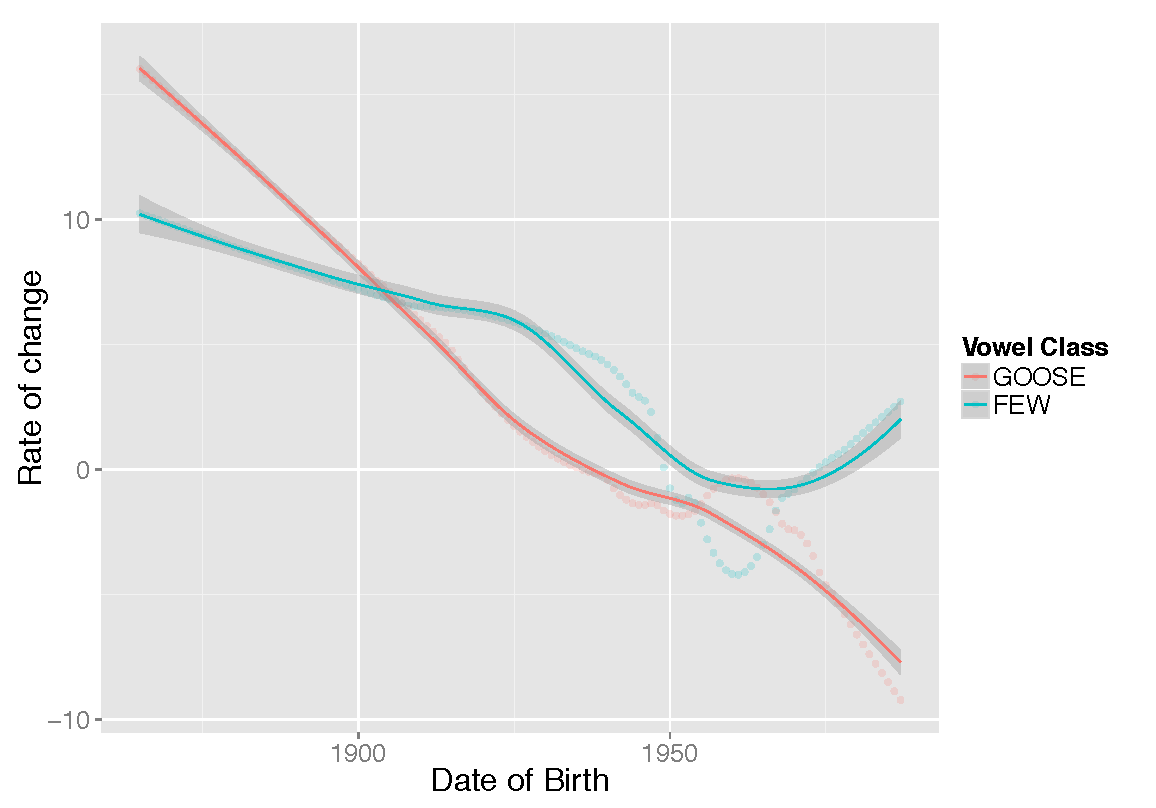
\includegraphics[width=.8\textwidth,height=.7\textheight]{NZEroc.pdf}
	\end{center}
	\end{block}	
\end{frame}

\section{Conclusions}

\begin{frame}{Conclusions: 3 types of allophonic splits}
	\begin{block}{Mechanical means}
		\begin{itemize}
			\item Effect of duration for the whole change until reanalysis
			\item Gradual split in rate of change \pause
		\end{itemize}
	\end{block}
	
	\begin{block}{Spontaneous phonologization}
		\begin{itemize}
			\item No effect of duration (pre-split don't have a distinction and post-split don't coarticulate)
			\item Immediate split in rate of change \pause
		\end{itemize}
	\end{block}
	
	\begin{block}{Phonological specialization}
		\begin{itemize}
			\item Effect of duration until reanalysis
			\item Immediate split in rate of change 
		\end{itemize}
	\end{block}
\end{frame}

\begin{frame}{Conclusions: Final thoughts}
	\begin{itemize}
		\item To use these metrics, we need \textbf{lots} of data from lots of people \pause
			\begin{itemize}
			\item We need data on changes before they happen \pause
			\end{itemize}
		\item DARLA, FAVE \pause
		\item What about suprasegmentals?
			\begin{itemize}
			\item Duration and ROC are good metrics for vocalic and consonantal change \pause
			\item \cite{Cho2015} Development of pitch contrast in Korean prosody \pause 
			\end{itemize}		
		\item Questions going further: how does allophone emergence relate to phoneme emergence?
	\end{itemize}
\end{frame}

\begin{frame}[allowframebreaks]
\frametitle{References}

%\newcommand*{\newblock}{natbib}
\bibliographystyle{linquiry2}
\bibliography{fwavrefs}
\end{frame}

\begin{frame}
\begin{center}
\huge{Thank you!}
\end{center}
\end{frame}

\end{document}